% %% %%%%%%%%%%%%%%%%%%%%%%%%%%%%%%%%%%%%%%%%%%%%%%%%%%%%%%%%%%
% practica.tex
%
% Author:  Mauricio Matamoros
% License: MIT
%
% %% %%%%%%%%%%%%%%%%%%%%%%%%%%%%%%%%%%%%%%%%%%%%%%%%%%%%%%%%%%

\documentclass[letterpaper,10.5pt]{article}
% %% %%%%%%%%%%%%%%%%%%%%%%%%%%%%%%%%%%%%%%%%%%%%%%%%%%%%%%%%%
%
% packages.tex
%
%  Author: Mauricio Matamoros
%  Date:   2020.02.28
%
%  Contiene la lista de paquetes requeridos para generar
%  el archivo-reporte de las prácticas de laboratorio
%
% %% %%%%%%%%%%%%%%%%%%%%%%%%%%%%%%%%%%%%%%%%%%%%%%%%%%%%%%%%%
% Archivo principal de LaTeX
%!TEX root = ../reporte.tex

\usepackage[utf8]{inputenc}                  % Soporte para utf8
\usepackage[T1]{fontenc}                     % Soporte extendido de caracteres unicode
\usepackage[english,spanish,mexico]{babel}   % Define el idioma del documento a español (México) con soporte para inglés
% Standard packages
\usepackage{float}                           % Imágenes flotantes en el documento
\usepackage{ifthen}                          % Soporte if-then en macros
\usepackage{xspace}                          % Soporte de autoespaciado en macros
\usepackage{xstring}                         % Operaciones con cadenas en macros
\usepackage{wrapfig}                         % Permite colocar texto al rededor de figuras y otros flotantes
\usepackage{booktabs}                        % Embellece tablas
\usepackage{csquotes}                        % Entrecomillado automático y manejo de citas textuales
\usepackage{fancyhdr}                        % Permite reconfigurar encabezado y pie de página
\usepackage{fancyvrb}                        % Define estilos para entornos Verbatim
\usepackage{geometry}                        % Permite reconfigurar la geometría del documento
\usepackage{graphicx}                        % Permite insertar imágenes en varios formatos
\usepackage{lastpage}                        % Referencia a la última página del documento
\usepackage{listings}                        % Define estilos para entornos de código de programación (sintaxis)
\usepackage{multicol}                        % Manejo de texto en varias columnas
\usepackage{tabularx}                        % Tablas con ancho de columna variable
\usepackage{algorithm}                       % Entorno para escribir algoritmos
\usepackage{algpseudocode}                   % Entorno para escribir algoritmos en pseudocódigo
\usepackage[justification=centering]{subcaption} % Permite imágenes en viñetas
\usepackage[all]{nowidow}                    % Control de viudas y huérfanas
\usepackage[inline]{enumitem}                % Añade opciones de configuración a listas
\usepackage[usenames,dvipsnames]{xcolor}     % Permite el uso de colores en el documento
% Referencing
\usepackage{varioref}                        % Gestión de referencias variables
\usepackage{hyperref}                        % Gestión de referencias e hipervínculos
\usepackage[noabbrev,nameinlink,spanish]{cleveref} % Gestión de referencias cruzadas inteligentes con hipervínculos
\usepackage[square, comma, numbers, sort&compress]{natbib} % Gestión de referencias bibliográficas


\newcommand{\lpar}{(}\newcommand{\rpar}{)} %CHKTEX 9
\newcommand{\IIC}{I\textsuperscript{2}C\xspace}
\newcommand{\GND}{\textsc{Gnd}\xspace}
\newcommand{\VCC}{\textsc{Vcc}\xspace}
\newcommand{\VDD}{\textsc{Vdd}\xspace}
\newcommand{\textbi}[1]{\textbf{\textit{#1}}}
\newcommand{\degreesC}[1]{%
	#1\textsuperscript{o}C\xspace{}%
}
\newcommand{\degreesF}[1]{%
	#1\textsuperscript{o}F\xspace{}%
}

% \newcommand{\VCC}{V\textsubscript{CC}\xspace{}}
% \newcommand{\GND}{\textsc{Gnd}\xspace{}}
% CHKTEX-FILE 26
% CHKTEX-FILE 36

\tcbuselibrary{most}
% \tcbuselibrary{listings,breakable}
% \usetikzlibrary{shadings,shadows}
% \usetikzlibrary{decorations.pathmorphing}
% \usetikzlibrary{patterns}
% \usetikzlibrary{spy}
% \usetikzlibrary{arrows.meta}

\newtcolorbox{importantbox}[1]{%
	enhanced,
	colback=red!5!white,%
	colframe=red!75!black,%
	fonttitle=\bfseries,%
	center title,
	title={#1},%
	drop fuzzy shadow
}


\newtcolorbox{greenbox}[1]{%
	enhanced,
	colback=Green!5!white,%
	colframe=Green!75!black,%
	fonttitle=\bfseries,%
	center title,
	title={#1},%
	drop fuzzy shadow
}

\newtcolorbox{marker}[1][]{%
	enhanced,
	before skip=2mm,after skip=3mm,
	boxrule=0.4pt,left=5mm,right=2mm,top=1mm,bottom=1mm,
	colback=yellow!50,
	colframe=yellow!20!black,
	sharp corners,rounded corners=southeast,arc is angular,arc=3mm,
%	underlay={%
%		\path[fill=tcbcolback!80!black] ([yshift=3mm]interior.south east)--++(-0.4,-0.1)--++(0.1,-0.2);
%		\path[draw=tcbcolframe,shorten <=-0.05mm,shorten >=-0.05mm] ([yshift=3mm]interior.south east)--++(-0.4,-0.1)--++(0.1,-0.2);
%		\path[fill=yellow!50!black,draw=none] (interior.south west) rectangle node[white]{\Huge\bfseries !} ([xshift=4mm]interior.north west);
%	},
	drop fuzzy shadow,#1
}

%CHKTEX-FILE 1
%CHKTEX-FILE 7
%CHKTEX-FILE 9
% Default fixed font does not support bold face
\DeclareFixedFont{\ttb}{T1}{txtt}{bx}{n}{8} % for bold
\DeclareFixedFont{\ttm}{T1}{txtt}{m}{n}{8}  % for normal

% Custom colors
\usepackage{color}
\definecolor{keywordsColor}{rgb}{0,0,0.5}
\definecolor{customColor}{rgb}{0.6,0,0}
\definecolor{stringColor}{rgb}{0,0.5,0}

% Code highlighting python
\renewcommand{\ttdefault}{pcr}
\lstset{
	language=Python,                              % the language of the code (can be overrided per snippet)
	backgroundcolor=\color{white},                % choose the background color
	basicstyle=\footnotesize\ttfamily,            % the size of the fonts that are used for the code
	breakatwhitespace=false,                      % sets if automatic breaks should only happen at whitespace
	breaklines=true,                              % sets automatic line breaking
	captionpos=t,                                 % sets the caption-position to bottom
	commentstyle=\color{gray},                    % comment style
	deletekeywords={},                            % if you want to delete keywords from the given language
%	escapeinside={\%*}{*)},                       % if you want to add LaTeX within your code
	extendedchars=true,                           % lets you use non-ASCII characters; for 8-bits encodings only, does not work with UTF-8
	frame=tb,                                     % adds a frame around the code
	keepspaces=true,                              % keeps spaces in text, useful for keeping indentation of code (possibly needs columns=flexible)
	keywordstyle=\color{keywordsColor}\bfseries,  % keyword style
	numbers=left,                                 % where to put the line-numbers; possible values are (none, left, right)
	numbersep=5pt,                                % how far the line-numbers are from the code
	numberstyle=\tiny\color{gray},                % the style that is used for the line-numbers
	rulecolor=\color{black},                      % if not set, the frame-color may be changed on line-breaks within not-black text (e.g. comments (green here))
	showspaces=false,                             % show spaces everywhere adding particular underscores; it overrides 'showstringspaces'
	showstringspaces=false,                       % underline spaces within strings only
	showtabs=false,                               % show tabs within strings adding particular underscores
	stepnumber=1,                                 % the step between two line-numbers. If it's 1, each line will be numbered
	stringstyle=\color{stringColor},              % string literal style
	tabsize=2,                                    % sets default tabsize to 2 spaces
	title=\lstname,                               % show the filename of files included with \lstinputlisting; also try caption instead of title
	columns=fixed,                                % Using fixed column width (for e.g. nice alignment)
	otherkeywords={self},                         % if you want to add more keywords to the set
	emphstyle=\color{customColor}\bfseries,       % Custom highlighting style
	emph={__init__,__main__,True,False,None},     % Custom highlighting keywords
	xleftmargin=1cm,                              % Left margin
	xrightmargin=1cm,                             % Right margin
	% Unicode compatibility
	inputencoding=utf8,
	literate={%
	            {Á}{{\'a}}1 {É}{{\'E}}1 {Í}{{\'I}}1 {Ó}{{\'O}}1 {Ú}{{\'U}}1%
	            {á}{{\'a}}1 {é}{{\'e}}1 {í}{{\'i}}1 {ó}{{\'o}}1 {ú}{{\'u}}1%
	            {À}{{\`A}}1 {È}{{\'E}}1 {Ì}{{\`I}}1 {Ò}{{\`O}}1 {Ù}{{\`U}}1%
	            {à}{{\`a}}1 {è}{{\`e}}1 {ì}{{\`i}}1 {ò}{{\`o}}1 {ù}{{\`u}}1%
	            {Ä}{{\"A}}1 {Ë}{{\"E}}1 {Ï}{{\"I}}1 {Ö}{{\"O}}1 {Ü}{{\"U}}1%
	            {ä}{{\"a}}1 {ë}{{\"e}}1 {ï}{{\"i}}1 {ö}{{\"o}}1 {ü}{{\"u}}1%
	            {Â}{{\^A}}1 {Ê}{{\^E}}1 {Î}{{\^I}}1 {Ô}{{\^O}}1 {Û}{{\^U}}1%
	            {â}{{\^a}}1 {ê}{{\^e}}1 {î}{{\^i}}1 {ô}{{\^o}}1 {û}{{\^u}}1% CHKTEX 19
	            {Ã}{{\~a}}1 {Ẽ}{{\~E}}1 {Ĩ}{{\~I}}1 {Õ}{{\~O}}1 {Ũ}{{\~U}}1 {Ñ}{{\~N}}1%
	            {ã}{{\~a}}1 {ẽ}{{\~e}}1 {ĩ}{{\~i}}1 {õ}{{\~o}}1 {ũ}{{\~u}}1 {ñ}{{\~n}}1%
	            {œ}{{\oe}}1 {Œ}{{\OE}}1 {æ}{{\ae}}1 {Æ}{{\AE}}1 {ß}{{\ss}}1%
	            {ç}{{\c c}}1 {Ç}{{\c C}}1 {ø}{{\o}}1 {å}{{\r a}}1 {Å}{{\r A}}1%
	            {€}{{\EUR}}1 {£}{{\pounds}}1 {×}{{\(\times\)}}1% CHKTEX 21
	            {°}{{\textsuperscript{o}}}1%
	            {¹}{{\textsuperscript{1}}}1%
	            {²}{{\textsuperscript{2}}}1%
	            {³}{{\textsuperscript{3}}}1%
	            {⁴}{{\textsuperscript{4}}}1% CHKTEX 19
	            {⁵}{{\textsuperscript{5}}}1% CHKTEX 19
	            {⁶}{{\textsuperscript{6}}}1% CHKTEX 19
	            {⁷}{{\textsuperscript{7}}}1% CHKTEX 19
	            {⁸}{{\textsuperscript{8}}}1% CHKTEX 19
	            {⁹}{{\textsuperscript{9}}}1% CHKTEX 19
	            {⁰}{{\textsuperscript{0}}}1% CHKTEX 19
%	            {A}{{\textAlpha}}1
	            {α}{{\textalpha}}1%
%	            {B}{{\textBeta}}1
	            {β}{{\textbeta}}1%
	            {Γ}{{\textGamma}}1
	            {γ}{{\textgamma}}1%
	            {Δ}{{\textDelta}}1
	            {δ}{{\textdelta}}1% CHKTEX 19
%	            {E}{{\textEpsilon}}1
	            {ϵ}{{\textepsilon}}1%
%	            {Z}{{\textZeta}}1
	            {ζ}{{\textzeta}}1%
%	            {H}{{\textEta}}1
	            {η}{{\texteta}}1%
	            {Θ}{{\textTheta}}1
	            {θ}{{\texttheta}}1%
%	            {I}{{\textIota}}1
	            {ι}{{\textiota}}1%
%	            {K}{{\textKappa}}1
	            {κ}{{\textkappa}}1%
	            {Λ}{{\textLambda}}1
	            {λ}{{\textlambda}}1%
%	            {M}{{\textMu}}1
	            {μ}{{\textmu}}1%
%	            {N}{{\textNu}}1
	            {ν}{{\textnu}}1%
	            {Ξ}{{\textXi}}1
	            {ξ}{{\textxi}}1%
%	            {O}{{\textOmikron}}1
%	            {o}{{\textomikron}}1%
	            {Π}{{\textPi}}1
	            {π}{{\textpi}}1%
%	            {P}{{\textRho}}1
	            {ρ}{{\textrho}}1%
	            {Σ}{{\textSigma}}1
	            {σ}{{\textsigma}}1%
%	            {T}{{\textTau}}1
	            {τ}{{\texttau}}1%
	            {ϒ}{{\textUpsilon}}1
	            {υ}{{\textupsilon}}1%
	            {Φ}{{\textPhi}}1
	            {ϕ}{{\textphi}}1%
%	            {X}{{\textChi}}1
	            {χ}{{\textchi}}1%
	            {Ψ}{{\textPsi}}1
	            {ψ}{{\textpsi}}1%
	            {Ω}{{\textOmega}}1
	            {ω}{{\textomega}}1%
	            {ζ}{{\varsigma}}1%
%	            {}{{\straightphi}}1%
%	            {}{{\scripttheta}}1%
%	            {}{{\straighttheta}}1%
%	            {}{{\straightepsilon}}1%
	         },
}

\lstdefinestyle{c_with_comments}%
{
	language     = c,
	morecomment  = [l]{//},
	morecomment  = [s]{/*}{*/},
	breaklines,
}

\lstdefinestyle{c_without_comments}{%
	style        = c_with_comments,
	% numbers      = none,
	% keepspaces   = false,
	morecomment  = [l][\nullfont]{//},
	morecomment  = [is]{//}{\^^M},
	morecomment  = [is]{/*}{*/},
	emptylines   = *1,
}

\lstdefinestyle{py_without_comments}{%
	language     = python,
	morecomment  = [l][\nullfont]{\#},
	% morecomment  = [il]{\#},
	% morecomment  = [is]{\#}{\^^M},
	emptylines   = *1,
}

\lstdefinestyle{py_without_doclines}{%
	morecomment  = [is]{'''}{'''},%CHKTEX 23
	morecomment  = [is]{"""}{"""},%CHKTEX 18
	morecomment  = [is]{\#'''}{'''},%CHKTEX 23
	morecomment  = [is]{\#"""}{"""},%CHKTEX 18
}

\lstdefinelanguage{conf}
{
	basicstyle=\ttfamily\small,
	columns=fullflexible,
	morecomment=[s][\color{Orchid}\bfseries]{[}{]},
	morecomment=[l]{\#},
	morecomment=[l]{;},
	commentstyle=\color{gray}\ttfamily,
	% morekeywords={},
	% otherkeywords={=,:},
	% keywordstyle={\color{Green}\bfseries}
}

% \captionsetup[lstlisting]{font={small,tt}}
\captionsetup[lstlisting]{%
	font={small},
}



\DefineVerbatimEnvironment{Verbatim}{Verbatim}{%
	fontsize=\footnotesize,%
	frame=leftline,%
	framesep=2em,    % separation between frame and text
}

\RecustomVerbatimCommand{\VerbatimInput}{VerbatimInput}{%
	fontsize=\footnotesize,
%	frame=lines,            % top and bottom rule only
	frame=leftline,         % left rule only
	numbers=left,           % Line numbers on the left
	numbersep=0.25em,       % Gap between numbers and verbatim lines
	xleftmargin=4em,        % Indentation to add at the start of each line
	xrightmargin=4em,       % Right margin to add after each line
	framesep=0.5em,         % separation between frame and text
	rulecolor=\color{Gray}, % Color of the lines
	labelposition=topline,  %
	samepage=false,         % When true, prevents verbatim environment from
	                        % being broken between pages
%	commandchars=\|\(\),    % escape character and argument delimiters for
	                        % commands within the verbatim
%	commentchar=*           % comment character
}


% CHKTEX-FILE 1
% CHKTEX-FILE 13
% CHKTEX-FILE 18
% CHKTEX-FILE 35
\documentclass[letterpaper,12pt,twocolumn]{article}
% Input encodign

% %% %%%%%%%%%%%%%%%%%%%%%%%%%%%%%%%%%%%%%%%%%%%%%%%%%%%%%%%%%
%
% packages.tex
%
%  Author: Mauricio Matamoros
%  Date:   2020.02.28
%
%  Contiene la lista de paquetes requeridos para generar
%  el archivo-reporte de las prácticas de laboratorio
%
% %% %%%%%%%%%%%%%%%%%%%%%%%%%%%%%%%%%%%%%%%%%%%%%%%%%%%%%%%%%
% Archivo principal de LaTeX
%!TEX root = ../reporte.tex

\usepackage[utf8]{inputenc}                  % Soporte para utf8
\usepackage[T1]{fontenc}                     % Soporte extendido de caracteres unicode
\usepackage[english,spanish,mexico]{babel}   % Define el idioma del documento a español (México) con soporte para inglés
% Standard packages
\usepackage{float}                           % Imágenes flotantes en el documento
\usepackage{ifthen}                          % Soporte if-then en macros
\usepackage{xspace}                          % Soporte de autoespaciado en macros
\usepackage{xstring}                         % Operaciones con cadenas en macros
\usepackage{wrapfig}                         % Permite colocar texto al rededor de figuras y otros flotantes
\usepackage{booktabs}                        % Embellece tablas
\usepackage{csquotes}                        % Entrecomillado automático y manejo de citas textuales
\usepackage{fancyhdr}                        % Permite reconfigurar encabezado y pie de página
\usepackage{fancyvrb}                        % Define estilos para entornos Verbatim
\usepackage{geometry}                        % Permite reconfigurar la geometría del documento
\usepackage{graphicx}                        % Permite insertar imágenes en varios formatos
\usepackage{lastpage}                        % Referencia a la última página del documento
\usepackage{listings}                        % Define estilos para entornos de código de programación (sintaxis)
\usepackage{multicol}                        % Manejo de texto en varias columnas
\usepackage{tabularx}                        % Tablas con ancho de columna variable
\usepackage{algorithm}                       % Entorno para escribir algoritmos
\usepackage{algpseudocode}                   % Entorno para escribir algoritmos en pseudocódigo
\usepackage[justification=centering]{subcaption} % Permite imágenes en viñetas
\usepackage[all]{nowidow}                    % Control de viudas y huérfanas
\usepackage[inline]{enumitem}                % Añade opciones de configuración a listas
\usepackage[usenames,dvipsnames]{xcolor}     % Permite el uso de colores en el documento
% Referencing
\usepackage{varioref}                        % Gestión de referencias variables
\usepackage{hyperref}                        % Gestión de referencias e hipervínculos
\usepackage[noabbrev,nameinlink,spanish]{cleveref} % Gestión de referencias cruzadas inteligentes con hipervínculos
\usepackage[square, comma, numbers, sort&compress]{natbib} % Gestión de referencias bibliográficas


\newcommand{\lpar}{(}\newcommand{\rpar}{)} %CHKTEX 9
\newcommand{\IIC}{I\textsuperscript{2}C\xspace}
\newcommand{\GND}{\textsc{Gnd}\xspace}
\newcommand{\VCC}{\textsc{Vcc}\xspace}
\newcommand{\VDD}{\textsc{Vdd}\xspace}
\newcommand{\textbi}[1]{\textbf{\textit{#1}}}
\newcommand{\degreesC}[1]{%
	#1\textsuperscript{o}C\xspace{}%
}
\newcommand{\degreesF}[1]{%
	#1\textsuperscript{o}F\xspace{}%
}

% \newcommand{\VCC}{V\textsubscript{CC}\xspace{}}
% \newcommand{\GND}{\textsc{Gnd}\xspace{}}
% CHKTEX-FILE 1
% CHKTEX-FILE 13
% CHKTEX-FILE 18
% CHKTEX-FILE 35
\documentclass[letterpaper,12pt,twocolumn]{article}
% Input encodign

% %% %%%%%%%%%%%%%%%%%%%%%%%%%%%%%%%%%%%%%%%%%%%%%%%%%%%%%%%%%
%
% packages.tex
%
%  Author: Mauricio Matamoros
%  Date:   2020.02.28
%
%  Contiene la lista de paquetes requeridos para generar
%  el archivo-reporte de las prácticas de laboratorio
%
% %% %%%%%%%%%%%%%%%%%%%%%%%%%%%%%%%%%%%%%%%%%%%%%%%%%%%%%%%%%
% Archivo principal de LaTeX
%!TEX root = ../reporte.tex

\usepackage[utf8]{inputenc}                  % Soporte para utf8
\usepackage[T1]{fontenc}                     % Soporte extendido de caracteres unicode
\usepackage[english,spanish,mexico]{babel}   % Define el idioma del documento a español (México) con soporte para inglés
% Standard packages
\usepackage{float}                           % Imágenes flotantes en el documento
\usepackage{ifthen}                          % Soporte if-then en macros
\usepackage{xspace}                          % Soporte de autoespaciado en macros
\usepackage{xstring}                         % Operaciones con cadenas en macros
\usepackage{wrapfig}                         % Permite colocar texto al rededor de figuras y otros flotantes
\usepackage{booktabs}                        % Embellece tablas
\usepackage{csquotes}                        % Entrecomillado automático y manejo de citas textuales
\usepackage{fancyhdr}                        % Permite reconfigurar encabezado y pie de página
\usepackage{fancyvrb}                        % Define estilos para entornos Verbatim
\usepackage{geometry}                        % Permite reconfigurar la geometría del documento
\usepackage{graphicx}                        % Permite insertar imágenes en varios formatos
\usepackage{lastpage}                        % Referencia a la última página del documento
\usepackage{listings}                        % Define estilos para entornos de código de programación (sintaxis)
\usepackage{multicol}                        % Manejo de texto en varias columnas
\usepackage{tabularx}                        % Tablas con ancho de columna variable
\usepackage{algorithm}                       % Entorno para escribir algoritmos
\usepackage{algpseudocode}                   % Entorno para escribir algoritmos en pseudocódigo
\usepackage[justification=centering]{subcaption} % Permite imágenes en viñetas
\usepackage[all]{nowidow}                    % Control de viudas y huérfanas
\usepackage[inline]{enumitem}                % Añade opciones de configuración a listas
\usepackage[usenames,dvipsnames]{xcolor}     % Permite el uso de colores en el documento
% Referencing
\usepackage{varioref}                        % Gestión de referencias variables
\usepackage{hyperref}                        % Gestión de referencias e hipervínculos
\usepackage[noabbrev,nameinlink,spanish]{cleveref} % Gestión de referencias cruzadas inteligentes con hipervínculos
\usepackage[square, comma, numbers, sort&compress]{natbib} % Gestión de referencias bibliográficas


\newcommand{\lpar}{(}\newcommand{\rpar}{)} %CHKTEX 9
\newcommand{\IIC}{I\textsuperscript{2}C\xspace}
\newcommand{\GND}{\textsc{Gnd}\xspace}
\newcommand{\VCC}{\textsc{Vcc}\xspace}
\newcommand{\VDD}{\textsc{Vdd}\xspace}
\newcommand{\textbi}[1]{\textbf{\textit{#1}}}
\newcommand{\degreesC}[1]{%
	#1\textsuperscript{o}C\xspace{}%
}
\newcommand{\degreesF}[1]{%
	#1\textsuperscript{o}F\xspace{}%
}

% \newcommand{\VCC}{V\textsubscript{CC}\xspace{}}
% \newcommand{\GND}{\textsc{Gnd}\xspace{}}
% CHKTEX-FILE 1
% CHKTEX-FILE 13
% CHKTEX-FILE 18
% CHKTEX-FILE 35
\documentclass[letterpaper,12pt,twocolumn]{article}
% Input encodign

\input{setup/packages}
\input{setup/macros}
\input{setup/document}
\input{setup/listings}

\author{\footnotesize Autor: José Mauricio Matamoros de Maria y Campos}
\title{Especificación para reportes de lectura}
\date{}


% Document body
\begin{document}
\maketitle

\section*{Reportes de lectura}
El objetivo de las lecturas asignadas como tarea es fomentar en el alumno el hábito de la lectura, tanto de documentos técnicos como literarios, ya sean estos en español o en inglés, además de incrementar las habilidades de comprensión de lectura, concreción de ideas, síntesis y redacción de texto en prosa.

Leer es muy importante en el aprendizaje pues la mayor parte de lo que se aprende se hace por medio de la lectura.
Cuando se quiere aprender algo, lo primero que se hace es leer.

Cuando se lee un texto con fines de estudio se resaltan las ideas importantes, se resume, se separan las ideas principales y se formulan cuestionarios para mejor comprender el texto. Cuando se lee por entretenimiento (por ejemplo un cuento o una novela), el texto se analiza y se relacionan hechos y situaciones a fin de poder disfrutar de él.

Un reporte de lectura es un informe escrito acerca del texto que se leyó.
Este informe debe contener los siguientes datos:

\begin{itemize}[noitemsep]
	\item Título del texto y nombre del autor
	\item Tema o asunto que trata
	\item Resumen, síntesis o reseña del texto
	\item Análisis crítico del contenido del texto
	\item Opinión personal del contenido de la lectura
	\item Conclusiones de la lectura
\end{itemize}

En el caso de texto literario no se espera un resumen, síntesis o reseña del texto, sino que deberá comentarse sobre la temática del mismo y resaltar los puntos más importantes, dejando claras sus impresiones y comentarios sobre el texto.

Tome en cuenta que ni la síntesis ni los resúmenes implican copiar y pegar párrafos enteros del texto. Lo importante es distinguir las ideas principales, hacerlas propias y (salvo que sean definiciones), parafrasearlas, es decir,  expresarlas en sus propias palabras.

Pasos para elaborar un reporte de lectura
\begin{enumerate}[noitemsep]
	\item Lea atentamente el texto. Evite distractores como música fuerte, televisión, teléfono, etc.
	\item Anote los términos y palabras que no conozca o entienda e investigue su significado en un diccionario.
	\item Una vez aclarados los términos desconocidos y palabras nuevas, vuelva a leer el texto para comprenderlo mejor.
	\item En la segunda lectura subraye o marque las ideas principales del texto.
	%Procure no escribir en los libros, especialmente si no le pertenecen. Si desea hacer anotaciones, utilice un lápiz blando y escriba con suavidad, o de preferencia use fotocopias.
	\item Tome las ideas principales, abstraígalas, analícelas y sólo entonces redacte su escrito.
\end{enumerate}
\end{document}

%CHKTEX-FILE 1
%CHKTEX-FILE 7
%CHKTEX-FILE 9
% Default fixed font does not support bold face
\DeclareFixedFont{\ttb}{T1}{txtt}{bx}{n}{8} % for bold
\DeclareFixedFont{\ttm}{T1}{txtt}{m}{n}{8}  % for normal

% Custom colors
\usepackage{color}
\definecolor{keywordsColor}{rgb}{0,0,0.5}
\definecolor{customColor}{rgb}{0.6,0,0}
\definecolor{stringColor}{rgb}{0,0.5,0}

% Code highlighting python
\renewcommand{\ttdefault}{pcr}
\lstset{
	language=Python,                              % the language of the code (can be overrided per snippet)
	backgroundcolor=\color{white},                % choose the background color
	basicstyle=\footnotesize\ttfamily,            % the size of the fonts that are used for the code
	breakatwhitespace=false,                      % sets if automatic breaks should only happen at whitespace
	breaklines=true,                              % sets automatic line breaking
	captionpos=t,                                 % sets the caption-position to bottom
	commentstyle=\color{gray},                    % comment style
	deletekeywords={},                            % if you want to delete keywords from the given language
%	escapeinside={\%*}{*)},                       % if you want to add LaTeX within your code
	extendedchars=true,                           % lets you use non-ASCII characters; for 8-bits encodings only, does not work with UTF-8
	frame=tb,                                     % adds a frame around the code
	keepspaces=true,                              % keeps spaces in text, useful for keeping indentation of code (possibly needs columns=flexible)
	keywordstyle=\color{keywordsColor}\bfseries,  % keyword style
	numbers=left,                                 % where to put the line-numbers; possible values are (none, left, right)
	numbersep=5pt,                                % how far the line-numbers are from the code
	numberstyle=\tiny\color{gray},                % the style that is used for the line-numbers
	rulecolor=\color{black},                      % if not set, the frame-color may be changed on line-breaks within not-black text (e.g. comments (green here))
	showspaces=false,                             % show spaces everywhere adding particular underscores; it overrides 'showstringspaces'
	showstringspaces=false,                       % underline spaces within strings only
	showtabs=false,                               % show tabs within strings adding particular underscores
	stepnumber=1,                                 % the step between two line-numbers. If it's 1, each line will be numbered
	stringstyle=\color{stringColor},              % string literal style
	tabsize=2,                                    % sets default tabsize to 2 spaces
	title=\lstname,                               % show the filename of files included with \lstinputlisting; also try caption instead of title
	columns=fixed,                                % Using fixed column width (for e.g. nice alignment)
	otherkeywords={self},                         % if you want to add more keywords to the set
	emphstyle=\color{customColor}\bfseries,       % Custom highlighting style
	emph={__init__,__main__,True,False,None},     % Custom highlighting keywords
	xleftmargin=1cm,                              % Left margin
	xrightmargin=1cm,                             % Right margin
	% Unicode compatibility
	inputencoding=utf8,
	literate={%
	            {Á}{{\'a}}1 {É}{{\'E}}1 {Í}{{\'I}}1 {Ó}{{\'O}}1 {Ú}{{\'U}}1%
	            {á}{{\'a}}1 {é}{{\'e}}1 {í}{{\'i}}1 {ó}{{\'o}}1 {ú}{{\'u}}1%
	            {À}{{\`A}}1 {È}{{\'E}}1 {Ì}{{\`I}}1 {Ò}{{\`O}}1 {Ù}{{\`U}}1%
	            {à}{{\`a}}1 {è}{{\`e}}1 {ì}{{\`i}}1 {ò}{{\`o}}1 {ù}{{\`u}}1%
	            {Ä}{{\"A}}1 {Ë}{{\"E}}1 {Ï}{{\"I}}1 {Ö}{{\"O}}1 {Ü}{{\"U}}1%
	            {ä}{{\"a}}1 {ë}{{\"e}}1 {ï}{{\"i}}1 {ö}{{\"o}}1 {ü}{{\"u}}1%
	            {Â}{{\^A}}1 {Ê}{{\^E}}1 {Î}{{\^I}}1 {Ô}{{\^O}}1 {Û}{{\^U}}1%
	            {â}{{\^a}}1 {ê}{{\^e}}1 {î}{{\^i}}1 {ô}{{\^o}}1 {û}{{\^u}}1% CHKTEX 19
	            {Ã}{{\~a}}1 {Ẽ}{{\~E}}1 {Ĩ}{{\~I}}1 {Õ}{{\~O}}1 {Ũ}{{\~U}}1 {Ñ}{{\~N}}1%
	            {ã}{{\~a}}1 {ẽ}{{\~e}}1 {ĩ}{{\~i}}1 {õ}{{\~o}}1 {ũ}{{\~u}}1 {ñ}{{\~n}}1%
	            {œ}{{\oe}}1 {Œ}{{\OE}}1 {æ}{{\ae}}1 {Æ}{{\AE}}1 {ß}{{\ss}}1%
	            {ç}{{\c c}}1 {Ç}{{\c C}}1 {ø}{{\o}}1 {å}{{\r a}}1 {Å}{{\r A}}1%
	            {€}{{\EUR}}1 {£}{{\pounds}}1 {×}{{\(\times\)}}1% CHKTEX 21
	            {°}{{\textsuperscript{o}}}1%
	            {¹}{{\textsuperscript{1}}}1%
	            {²}{{\textsuperscript{2}}}1%
	            {³}{{\textsuperscript{3}}}1%
	            {⁴}{{\textsuperscript{4}}}1% CHKTEX 19
	            {⁵}{{\textsuperscript{5}}}1% CHKTEX 19
	            {⁶}{{\textsuperscript{6}}}1% CHKTEX 19
	            {⁷}{{\textsuperscript{7}}}1% CHKTEX 19
	            {⁸}{{\textsuperscript{8}}}1% CHKTEX 19
	            {⁹}{{\textsuperscript{9}}}1% CHKTEX 19
	            {⁰}{{\textsuperscript{0}}}1% CHKTEX 19
%	            {A}{{\textAlpha}}1
	            {α}{{\textalpha}}1%
%	            {B}{{\textBeta}}1
	            {β}{{\textbeta}}1%
	            {Γ}{{\textGamma}}1
	            {γ}{{\textgamma}}1%
	            {Δ}{{\textDelta}}1
	            {δ}{{\textdelta}}1% CHKTEX 19
%	            {E}{{\textEpsilon}}1
	            {ϵ}{{\textepsilon}}1%
%	            {Z}{{\textZeta}}1
	            {ζ}{{\textzeta}}1%
%	            {H}{{\textEta}}1
	            {η}{{\texteta}}1%
	            {Θ}{{\textTheta}}1
	            {θ}{{\texttheta}}1%
%	            {I}{{\textIota}}1
	            {ι}{{\textiota}}1%
%	            {K}{{\textKappa}}1
	            {κ}{{\textkappa}}1%
	            {Λ}{{\textLambda}}1
	            {λ}{{\textlambda}}1%
%	            {M}{{\textMu}}1
	            {μ}{{\textmu}}1%
%	            {N}{{\textNu}}1
	            {ν}{{\textnu}}1%
	            {Ξ}{{\textXi}}1
	            {ξ}{{\textxi}}1%
%	            {O}{{\textOmikron}}1
%	            {o}{{\textomikron}}1%
	            {Π}{{\textPi}}1
	            {π}{{\textpi}}1%
%	            {P}{{\textRho}}1
	            {ρ}{{\textrho}}1%
	            {Σ}{{\textSigma}}1
	            {σ}{{\textsigma}}1%
%	            {T}{{\textTau}}1
	            {τ}{{\texttau}}1%
	            {ϒ}{{\textUpsilon}}1
	            {υ}{{\textupsilon}}1%
	            {Φ}{{\textPhi}}1
	            {ϕ}{{\textphi}}1%
%	            {X}{{\textChi}}1
	            {χ}{{\textchi}}1%
	            {Ψ}{{\textPsi}}1
	            {ψ}{{\textpsi}}1%
	            {Ω}{{\textOmega}}1
	            {ω}{{\textomega}}1%
	            {ζ}{{\varsigma}}1%
%	            {}{{\straightphi}}1%
%	            {}{{\scripttheta}}1%
%	            {}{{\straighttheta}}1%
%	            {}{{\straightepsilon}}1%
	         },
}

\lstdefinestyle{c_with_comments}%
{
	language     = c,
	morecomment  = [l]{//},
	morecomment  = [s]{/*}{*/},
	breaklines,
}

\lstdefinestyle{c_without_comments}{%
	style        = c_with_comments,
	% numbers      = none,
	% keepspaces   = false,
	morecomment  = [l][\nullfont]{//},
	morecomment  = [is]{//}{\^^M},
	morecomment  = [is]{/*}{*/},
	emptylines   = *1,
}

\lstdefinestyle{py_without_comments}{%
	language     = python,
	morecomment  = [l][\nullfont]{\#},
	% morecomment  = [il]{\#},
	% morecomment  = [is]{\#}{\^^M},
	emptylines   = *1,
}

\lstdefinestyle{py_without_doclines}{%
	morecomment  = [is]{'''}{'''},%CHKTEX 23
	morecomment  = [is]{"""}{"""},%CHKTEX 18
	morecomment  = [is]{\#'''}{'''},%CHKTEX 23
	morecomment  = [is]{\#"""}{"""},%CHKTEX 18
}

\lstdefinelanguage{conf}
{
	basicstyle=\ttfamily\small,
	columns=fullflexible,
	morecomment=[s][\color{Orchid}\bfseries]{[}{]},
	morecomment=[l]{\#},
	morecomment=[l]{;},
	commentstyle=\color{gray}\ttfamily,
	% morekeywords={},
	% otherkeywords={=,:},
	% keywordstyle={\color{Green}\bfseries}
}

% \captionsetup[lstlisting]{font={small,tt}}
\captionsetup[lstlisting]{%
	font={small},
}



\DefineVerbatimEnvironment{Verbatim}{Verbatim}{%
	fontsize=\footnotesize,%
	frame=leftline,%
	framesep=2em,    % separation between frame and text
}

\RecustomVerbatimCommand{\VerbatimInput}{VerbatimInput}{%
	fontsize=\footnotesize,
%	frame=lines,            % top and bottom rule only
	frame=leftline,         % left rule only
	numbers=left,           % Line numbers on the left
	numbersep=0.25em,       % Gap between numbers and verbatim lines
	xleftmargin=4em,        % Indentation to add at the start of each line
	xrightmargin=4em,       % Right margin to add after each line
	framesep=0.5em,         % separation between frame and text
	rulecolor=\color{Gray}, % Color of the lines
	labelposition=topline,  %
	samepage=false,         % When true, prevents verbatim environment from
	                        % being broken between pages
%	commandchars=\|\(\),    % escape character and argument delimiters for
	                        % commands within the verbatim
%	commentchar=*           % comment character
}



\author{\footnotesize Autor: José Mauricio Matamoros de Maria y Campos}
\title{Especificación para reportes de lectura}
\date{}


% Document body
\begin{document}
\maketitle

\section*{Reportes de lectura}
El objetivo de las lecturas asignadas como tarea es fomentar en el alumno el hábito de la lectura, tanto de documentos técnicos como literarios, ya sean estos en español o en inglés, además de incrementar las habilidades de comprensión de lectura, concreción de ideas, síntesis y redacción de texto en prosa.

Leer es muy importante en el aprendizaje pues la mayor parte de lo que se aprende se hace por medio de la lectura.
Cuando se quiere aprender algo, lo primero que se hace es leer.

Cuando se lee un texto con fines de estudio se resaltan las ideas importantes, se resume, se separan las ideas principales y se formulan cuestionarios para mejor comprender el texto. Cuando se lee por entretenimiento (por ejemplo un cuento o una novela), el texto se analiza y se relacionan hechos y situaciones a fin de poder disfrutar de él.

Un reporte de lectura es un informe escrito acerca del texto que se leyó.
Este informe debe contener los siguientes datos:

\begin{itemize}[noitemsep]
	\item Título del texto y nombre del autor
	\item Tema o asunto que trata
	\item Resumen, síntesis o reseña del texto
	\item Análisis crítico del contenido del texto
	\item Opinión personal del contenido de la lectura
	\item Conclusiones de la lectura
\end{itemize}

En el caso de texto literario no se espera un resumen, síntesis o reseña del texto, sino que deberá comentarse sobre la temática del mismo y resaltar los puntos más importantes, dejando claras sus impresiones y comentarios sobre el texto.

Tome en cuenta que ni la síntesis ni los resúmenes implican copiar y pegar párrafos enteros del texto. Lo importante es distinguir las ideas principales, hacerlas propias y (salvo que sean definiciones), parafrasearlas, es decir,  expresarlas en sus propias palabras.

Pasos para elaborar un reporte de lectura
\begin{enumerate}[noitemsep]
	\item Lea atentamente el texto. Evite distractores como música fuerte, televisión, teléfono, etc.
	\item Anote los términos y palabras que no conozca o entienda e investigue su significado en un diccionario.
	\item Una vez aclarados los términos desconocidos y palabras nuevas, vuelva a leer el texto para comprenderlo mejor.
	\item En la segunda lectura subraye o marque las ideas principales del texto.
	%Procure no escribir en los libros, especialmente si no le pertenecen. Si desea hacer anotaciones, utilice un lápiz blando y escriba con suavidad, o de preferencia use fotocopias.
	\item Tome las ideas principales, abstraígalas, analícelas y sólo entonces redacte su escrito.
\end{enumerate}
\end{document}

%CHKTEX-FILE 1
%CHKTEX-FILE 7
%CHKTEX-FILE 9
% Default fixed font does not support bold face
\DeclareFixedFont{\ttb}{T1}{txtt}{bx}{n}{8} % for bold
\DeclareFixedFont{\ttm}{T1}{txtt}{m}{n}{8}  % for normal

% Custom colors
\usepackage{color}
\definecolor{keywordsColor}{rgb}{0,0,0.5}
\definecolor{customColor}{rgb}{0.6,0,0}
\definecolor{stringColor}{rgb}{0,0.5,0}

% Code highlighting python
\renewcommand{\ttdefault}{pcr}
\lstset{
	language=Python,                              % the language of the code (can be overrided per snippet)
	backgroundcolor=\color{white},                % choose the background color
	basicstyle=\footnotesize\ttfamily,            % the size of the fonts that are used for the code
	breakatwhitespace=false,                      % sets if automatic breaks should only happen at whitespace
	breaklines=true,                              % sets automatic line breaking
	captionpos=t,                                 % sets the caption-position to bottom
	commentstyle=\color{gray},                    % comment style
	deletekeywords={},                            % if you want to delete keywords from the given language
%	escapeinside={\%*}{*)},                       % if you want to add LaTeX within your code
	extendedchars=true,                           % lets you use non-ASCII characters; for 8-bits encodings only, does not work with UTF-8
	frame=tb,                                     % adds a frame around the code
	keepspaces=true,                              % keeps spaces in text, useful for keeping indentation of code (possibly needs columns=flexible)
	keywordstyle=\color{keywordsColor}\bfseries,  % keyword style
	numbers=left,                                 % where to put the line-numbers; possible values are (none, left, right)
	numbersep=5pt,                                % how far the line-numbers are from the code
	numberstyle=\tiny\color{gray},                % the style that is used for the line-numbers
	rulecolor=\color{black},                      % if not set, the frame-color may be changed on line-breaks within not-black text (e.g. comments (green here))
	showspaces=false,                             % show spaces everywhere adding particular underscores; it overrides 'showstringspaces'
	showstringspaces=false,                       % underline spaces within strings only
	showtabs=false,                               % show tabs within strings adding particular underscores
	stepnumber=1,                                 % the step between two line-numbers. If it's 1, each line will be numbered
	stringstyle=\color{stringColor},              % string literal style
	tabsize=2,                                    % sets default tabsize to 2 spaces
	title=\lstname,                               % show the filename of files included with \lstinputlisting; also try caption instead of title
	columns=fixed,                                % Using fixed column width (for e.g. nice alignment)
	otherkeywords={self},                         % if you want to add more keywords to the set
	emphstyle=\color{customColor}\bfseries,       % Custom highlighting style
	emph={__init__,__main__,True,False,None},     % Custom highlighting keywords
	xleftmargin=1cm,                              % Left margin
	xrightmargin=1cm,                             % Right margin
	% Unicode compatibility
	inputencoding=utf8,
	literate={%
	            {Á}{{\'a}}1 {É}{{\'E}}1 {Í}{{\'I}}1 {Ó}{{\'O}}1 {Ú}{{\'U}}1%
	            {á}{{\'a}}1 {é}{{\'e}}1 {í}{{\'i}}1 {ó}{{\'o}}1 {ú}{{\'u}}1%
	            {À}{{\`A}}1 {È}{{\'E}}1 {Ì}{{\`I}}1 {Ò}{{\`O}}1 {Ù}{{\`U}}1%
	            {à}{{\`a}}1 {è}{{\`e}}1 {ì}{{\`i}}1 {ò}{{\`o}}1 {ù}{{\`u}}1%
	            {Ä}{{\"A}}1 {Ë}{{\"E}}1 {Ï}{{\"I}}1 {Ö}{{\"O}}1 {Ü}{{\"U}}1%
	            {ä}{{\"a}}1 {ë}{{\"e}}1 {ï}{{\"i}}1 {ö}{{\"o}}1 {ü}{{\"u}}1%
	            {Â}{{\^A}}1 {Ê}{{\^E}}1 {Î}{{\^I}}1 {Ô}{{\^O}}1 {Û}{{\^U}}1%
	            {â}{{\^a}}1 {ê}{{\^e}}1 {î}{{\^i}}1 {ô}{{\^o}}1 {û}{{\^u}}1% CHKTEX 19
	            {Ã}{{\~a}}1 {Ẽ}{{\~E}}1 {Ĩ}{{\~I}}1 {Õ}{{\~O}}1 {Ũ}{{\~U}}1 {Ñ}{{\~N}}1%
	            {ã}{{\~a}}1 {ẽ}{{\~e}}1 {ĩ}{{\~i}}1 {õ}{{\~o}}1 {ũ}{{\~u}}1 {ñ}{{\~n}}1%
	            {œ}{{\oe}}1 {Œ}{{\OE}}1 {æ}{{\ae}}1 {Æ}{{\AE}}1 {ß}{{\ss}}1%
	            {ç}{{\c c}}1 {Ç}{{\c C}}1 {ø}{{\o}}1 {å}{{\r a}}1 {Å}{{\r A}}1%
	            {€}{{\EUR}}1 {£}{{\pounds}}1 {×}{{\(\times\)}}1% CHKTEX 21
	            {°}{{\textsuperscript{o}}}1%
	            {¹}{{\textsuperscript{1}}}1%
	            {²}{{\textsuperscript{2}}}1%
	            {³}{{\textsuperscript{3}}}1%
	            {⁴}{{\textsuperscript{4}}}1% CHKTEX 19
	            {⁵}{{\textsuperscript{5}}}1% CHKTEX 19
	            {⁶}{{\textsuperscript{6}}}1% CHKTEX 19
	            {⁷}{{\textsuperscript{7}}}1% CHKTEX 19
	            {⁸}{{\textsuperscript{8}}}1% CHKTEX 19
	            {⁹}{{\textsuperscript{9}}}1% CHKTEX 19
	            {⁰}{{\textsuperscript{0}}}1% CHKTEX 19
%	            {A}{{\textAlpha}}1
	            {α}{{\textalpha}}1%
%	            {B}{{\textBeta}}1
	            {β}{{\textbeta}}1%
	            {Γ}{{\textGamma}}1
	            {γ}{{\textgamma}}1%
	            {Δ}{{\textDelta}}1
	            {δ}{{\textdelta}}1% CHKTEX 19
%	            {E}{{\textEpsilon}}1
	            {ϵ}{{\textepsilon}}1%
%	            {Z}{{\textZeta}}1
	            {ζ}{{\textzeta}}1%
%	            {H}{{\textEta}}1
	            {η}{{\texteta}}1%
	            {Θ}{{\textTheta}}1
	            {θ}{{\texttheta}}1%
%	            {I}{{\textIota}}1
	            {ι}{{\textiota}}1%
%	            {K}{{\textKappa}}1
	            {κ}{{\textkappa}}1%
	            {Λ}{{\textLambda}}1
	            {λ}{{\textlambda}}1%
%	            {M}{{\textMu}}1
	            {μ}{{\textmu}}1%
%	            {N}{{\textNu}}1
	            {ν}{{\textnu}}1%
	            {Ξ}{{\textXi}}1
	            {ξ}{{\textxi}}1%
%	            {O}{{\textOmikron}}1
%	            {o}{{\textomikron}}1%
	            {Π}{{\textPi}}1
	            {π}{{\textpi}}1%
%	            {P}{{\textRho}}1
	            {ρ}{{\textrho}}1%
	            {Σ}{{\textSigma}}1
	            {σ}{{\textsigma}}1%
%	            {T}{{\textTau}}1
	            {τ}{{\texttau}}1%
	            {ϒ}{{\textUpsilon}}1
	            {υ}{{\textupsilon}}1%
	            {Φ}{{\textPhi}}1
	            {ϕ}{{\textphi}}1%
%	            {X}{{\textChi}}1
	            {χ}{{\textchi}}1%
	            {Ψ}{{\textPsi}}1
	            {ψ}{{\textpsi}}1%
	            {Ω}{{\textOmega}}1
	            {ω}{{\textomega}}1%
	            {ζ}{{\varsigma}}1%
%	            {}{{\straightphi}}1%
%	            {}{{\scripttheta}}1%
%	            {}{{\straighttheta}}1%
%	            {}{{\straightepsilon}}1%
	         },
}

\lstdefinestyle{c_with_comments}%
{
	language     = c,
	morecomment  = [l]{//},
	morecomment  = [s]{/*}{*/},
	breaklines,
}

\lstdefinestyle{c_without_comments}{%
	style        = c_with_comments,
	% numbers      = none,
	% keepspaces   = false,
	morecomment  = [l][\nullfont]{//},
	morecomment  = [is]{//}{\^^M},
	morecomment  = [is]{/*}{*/},
	emptylines   = *1,
}

\lstdefinestyle{py_without_comments}{%
	language     = python,
	morecomment  = [l][\nullfont]{\#},
	% morecomment  = [il]{\#},
	% morecomment  = [is]{\#}{\^^M},
	emptylines   = *1,
}

\lstdefinestyle{py_without_doclines}{%
	morecomment  = [is]{'''}{'''},%CHKTEX 23
	morecomment  = [is]{"""}{"""},%CHKTEX 18
	morecomment  = [is]{\#'''}{'''},%CHKTEX 23
	morecomment  = [is]{\#"""}{"""},%CHKTEX 18
}

\lstdefinelanguage{conf}
{
	basicstyle=\ttfamily\small,
	columns=fullflexible,
	morecomment=[s][\color{Orchid}\bfseries]{[}{]},
	morecomment=[l]{\#},
	morecomment=[l]{;},
	commentstyle=\color{gray}\ttfamily,
	% morekeywords={},
	% otherkeywords={=,:},
	% keywordstyle={\color{Green}\bfseries}
}

% \captionsetup[lstlisting]{font={small,tt}}
\captionsetup[lstlisting]{%
	font={small},
}



\DefineVerbatimEnvironment{Verbatim}{Verbatim}{%
	fontsize=\footnotesize,%
	frame=leftline,%
	framesep=2em,    % separation between frame and text
}

\RecustomVerbatimCommand{\VerbatimInput}{VerbatimInput}{%
	fontsize=\footnotesize,
%	frame=lines,            % top and bottom rule only
	frame=leftline,         % left rule only
	numbers=left,           % Line numbers on the left
	numbersep=0.25em,       % Gap between numbers and verbatim lines
	xleftmargin=4em,        % Indentation to add at the start of each line
	xrightmargin=4em,       % Right margin to add after each line
	framesep=0.5em,         % separation between frame and text
	rulecolor=\color{Gray}, % Color of the lines
	labelposition=topline,  %
	samepage=false,         % When true, prevents verbatim environment from
	                        % being broken between pages
%	commandchars=\|\(\),    % escape character and argument delimiters for
	                        % commands within the verbatim
%	commentchar=*           % comment character
}



\author{\footnotesize Autor: José Mauricio Matamoros de Maria y Campos}
\title{Especificación para reportes de lectura}
\date{}


% Document body
\begin{document}
\maketitle

\section*{Reportes de lectura}
El objetivo de las lecturas asignadas como tarea es fomentar en el alumno el hábito de la lectura, tanto de documentos técnicos como literarios, ya sean estos en español o en inglés, además de incrementar las habilidades de comprensión de lectura, concreción de ideas, síntesis y redacción de texto en prosa.

Leer es muy importante en el aprendizaje pues la mayor parte de lo que se aprende se hace por medio de la lectura.
Cuando se quiere aprender algo, lo primero que se hace es leer.

Cuando se lee un texto con fines de estudio se resaltan las ideas importantes, se resume, se separan las ideas principales y se formulan cuestionarios para mejor comprender el texto. Cuando se lee por entretenimiento (por ejemplo un cuento o una novela), el texto se analiza y se relacionan hechos y situaciones a fin de poder disfrutar de él.

Un reporte de lectura es un informe escrito acerca del texto que se leyó.
Este informe debe contener los siguientes datos:

\begin{itemize}[noitemsep]
	\item Título del texto y nombre del autor
	\item Tema o asunto que trata
	\item Resumen, síntesis o reseña del texto
	\item Análisis crítico del contenido del texto
	\item Opinión personal del contenido de la lectura
	\item Conclusiones de la lectura
\end{itemize}

En el caso de texto literario no se espera un resumen, síntesis o reseña del texto, sino que deberá comentarse sobre la temática del mismo y resaltar los puntos más importantes, dejando claras sus impresiones y comentarios sobre el texto.

Tome en cuenta que ni la síntesis ni los resúmenes implican copiar y pegar párrafos enteros del texto. Lo importante es distinguir las ideas principales, hacerlas propias y (salvo que sean definiciones), parafrasearlas, es decir,  expresarlas en sus propias palabras.

Pasos para elaborar un reporte de lectura
\begin{enumerate}[noitemsep]
	\item Lea atentamente el texto. Evite distractores como música fuerte, televisión, teléfono, etc.
	\item Anote los términos y palabras que no conozca o entienda e investigue su significado en un diccionario.
	\item Una vez aclarados los términos desconocidos y palabras nuevas, vuelva a leer el texto para comprenderlo mejor.
	\item En la segunda lectura subraye o marque las ideas principales del texto.
	%Procure no escribir en los libros, especialmente si no le pertenecen. Si desea hacer anotaciones, utilice un lápiz blando y escriba con suavidad, o de preferencia use fotocopias.
	\item Tome las ideas principales, abstraígalas, analícelas y sólo entonces redacte su escrito.
\end{enumerate}
\end{document}


\author{\footnotesize Autor: José Mauricio Matamoros de Maria y Campos}
\title{Práctica 2 bis:\\Instalación de \emph{Android Open Source Project}\\
(LineageOS) en la Raspberry Pi\\
{\large Fundamentos de Sistemas Embebidos}}
\date{}


% Document body
\begin{document}
\maketitle

\section{Objetivo}%
\label{sec:objective}
El alumno aprenderá a instalar un sistema operativo de código abierto basado en Android en una tarjeta microcontroladora.

\section{Introducción}%
\label{sec:introduction}
LineageOS es un sistema operativo basado en Android diseñado para operar teléfonos inteligentes, tabletas y kiosocos, entre otros dispositivos móviles.
A diferencia del Android original que requiere de una licencia y ser compilado desde código fuente (approx 250GB más 150GB para su compilación), LineageOS ha sido adaptado para usar software gratuito y de código abierto casi de manera exclusiva.

Al estar diseñados para operar en un dispositivo táctil, suele decirse que los sistemas operativos basados en Android requieren de una pantalla tipo \emph{TouchScreen}.
Si bien esta afirmación no es cierta, la experiencia de usuario no será tan fluida con un teclado y un mouse como si se tuviera una pantalla táctil.

\section{Instrucciones}%
\label{sec:instructions}

Instalar LineageOS en la Raspberry Pi es relativamente sencillo.
Basta con descargar LineageOS y grabar la imagen de disco en una tarjeta de memoria microSD, desde la cual arrancará el sistema operativo.

Para esta práctica se necesitará:
\begin{itemize}[nosep]
	\item Una tarjeta de memoria microSD de al menos 8 GB (se recomiendan 16GB)
	\item Una computadora capaz de leer y escribir tarjetas microSD (o bien un adaptador para la misma) y conexión a internet para descargar la imagen de LineageOS. %CHKTEX 13
	\item Una Raspberry Pi 3B o posterior con al menos 2GB de memoria RAM
	\item Un monitor con soporte para HDMI
	\item Un teclado USB
	\item Un mouse USB
	\item Una memoria USB con formato \textsc{Fat32}
	\item Una fuente de alimentación de 5V@1A con adaptador microUSB o USB-C
\end{itemize}

\paragraph*{Importante:} Si no cuenta con monitor, teclado y mouse, no será posible instalar LineageOS en la Raspberry Pi.

% %% %%%%%%%%%%%%%%%%%%%%%%%%%%%%%%%%%%%%%%%%%%%%%%%%%%%%%%%%%%%%%%%%%%
%
% Step 1
%
% %% %%%%%%%%%%%%%%%%%%%%%%%%%%%%%%%%%%%%%%%%%%%%%%%%%%%%%%%%%%%%%%%%%%
\subsection{Paso 1: Descargar LineageOS}%
\label{sec:step1}
Ingrese a \url{https://konstakang.com/} y seleccione el modelo de su Raspberry (véase \Cref{fig:lineage-download}).
A continuación seleccione

\begin{figure}[H]
	\centering%
	\begin{subfigure}[b]{0.5\linewidth}
		\centering
		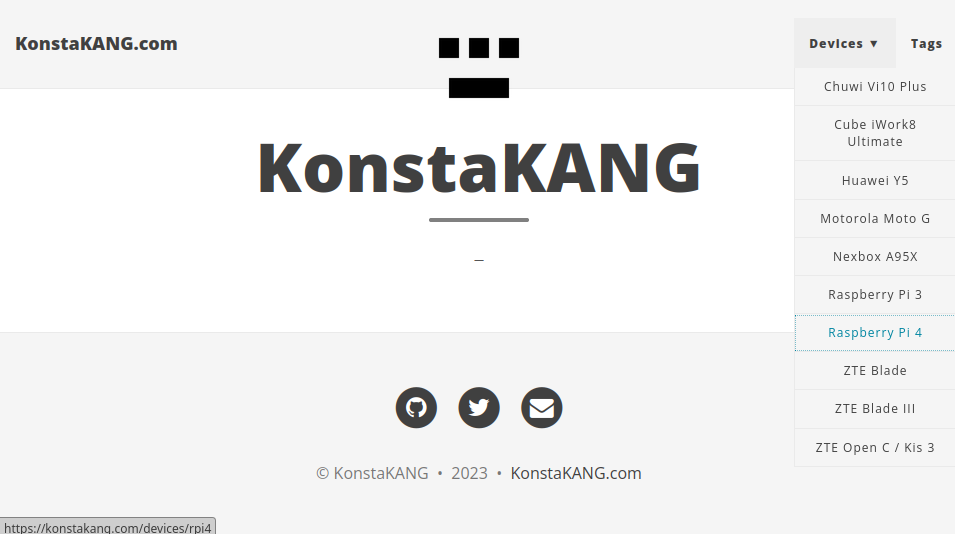
\includegraphics[width=0.9\linewidth,height=8cm,keepaspectratio]{img/p02-01a.png} %CHKTEX 8
		\caption{Página de KonstaKANG}
		\label{fig:konstaKANG-web} %CHKTEX 24
	\end{subfigure}%
	\begin{subfigure}[b]{0.5\linewidth}
		\centering
		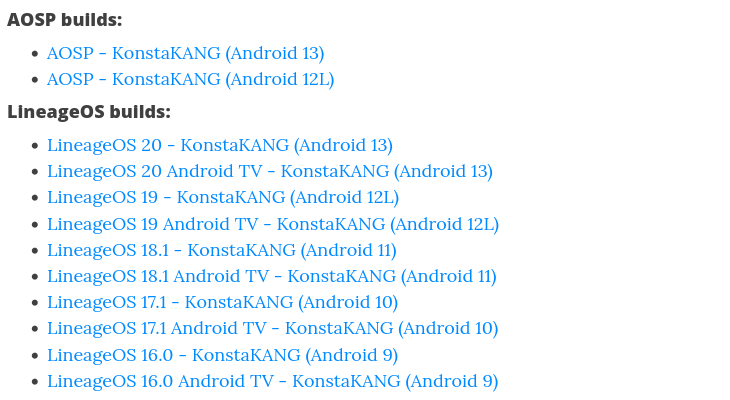
\includegraphics[width=0.9\linewidth,height=8cm,keepaspectratio]{img/p02-01b.png} %CHKTEX 8
		\caption{Versiones disponibles de Android LineageOS}
		\label{fig:lineage-flavors} %CHKTEX 24
	\end{subfigure}
	\caption{Descarga de LineageOS/KonstaKANG}%
	\label{fig:lineage-download} %CHKTEX 24
\end{figure}

La versión a descargar dependerá de la capacidad de la memoria microSD, la cantidad de recursos de la Raspberry y el uso que se le dará a la tarjeta microcontroladora.
Se recomienda descargar LineageOS 20.0 para la Raspberry Pi 4.

Ligas de acceso rápido se proporcionan a continuación por conveniencia:

\begin{itemize}[noitemsep]
	\item \href{https://www.androidfilehost.com/?fid=4279422670115708605}{LineageOS 20.0 para Raspberry Pi 4}
	\item \href{https://www.androidfilehost.com/?fid=10763459528675579938}{LineageOS 17.1 para Raspbrerry Pi 3B}
\end{itemize}


% %% %%%%%%%%%%%%%%%%%%%%%%%%%%%%%%%%%%%%%%%%%%%%%%%%%%%%%%%%%%%%%%%%%%
%
% Step 2
%
% %% %%%%%%%%%%%%%%%%%%%%%%%%%%%%%%%%%%%%%%%%%%%%%%%%%%%%%%%%%%%%%%%%%%
\subsection{Paso 2: Descargar NikGapps}%
Debido a que la Raspberry Pi no se considera un dispositivo comercializable con Android licenciable (no existe una compañía que pague a Google por el soporte de hardware y la licencia de acceso a la tienda de aplicaciones), LineageOS no viene con la tienda Google Play precargada.
Es por esto que es necesario instalar una tienda alternativa.

Dos de las opciones más cómunes son \emph{OpenGapps} y \emph{NikGapps}.
\emph{OpenGapps} se considera un desarrollo abandonado pues no actualizan las aplicaciones muy seguido o, si lo hacen, las actualizaciones se liberan con meses o incluso años de retraso.
Por otro lado, \emph{NikGapps} se actualiza con mucha más frecuencia.

Es por esto que se recomienda descargar \emph{NikGapps} de \url{https://nikgapps.com/}.
Para ello, simplemente acceda al sitio y, bajo descargas, encontrará un enlace que le llevará al sitio en SourceForge de donde podrá descargar la versión que más le convenga.
Siga los siguientes pasos:
\begin{enumerate}[nosep]
	\item De click en \emph{Download Now}.
	\item Una vez en SourceForge, vaya a \emph{Releases} y abra la carpeta con fecha más reciente.

\end{enumerate}
    Click on the links, then “Download Now”.
    On SourceForge, go to “Releases” and open the latest folder.

    Download the version you want, the “Core” package is enough for a Raspberry Pi, the important part is Google Play Store.

I recommend copying the “NikGapps” or “OpenGapps” file to a USB key.
It’s easier than downloading it from the Android system. I’ll show you in the last part how to install them. Attention: make sure the USB key is formatted in FAT32. It won’t work with another file format.


% %% %%%%%%%%%%%%%%%%%%%%%%%%%%%%%%%%%%%%%%%%%%%%%%%%%%%%%%%%%%%%%%%%%%
%
% Step 3
%
% %% %%%%%%%%%%%%%%%%%%%%%%%%%%%%%%%%%%%%%%%%%%%%%%%%%%%%%%%%%%%%%%%%%%
\subsection{Paso 3: Escribir imagen en la microSD}%
\label{sec:step2}
Si no lo ha hecho, introduzca la memoria microSD en la computadora.
La memoria será reformateada por lo que se aconseja respaldar la información.

Escribir la imagen de LineageOS en la microSD requiere de un programa externo según el sistema operativo.

% %% %%%%%%%%%%%%%%%%%%%%%%%%%%%%%%%%%%%%%%%%%%%%%%%%%%%%%%%%%%%%%%%%%%
%
% Step 3a: Linux
%
% %% %%%%%%%%%%%%%%%%%%%%%%%%%%%%%%%%%%%%%%%%%%%%%%%%%%%%%%%%%%%%%%%%%%
% \subsubsection{Escribir imagen usando Linux}%
Descargue \href{https://etcher.io/}{Etcher} en \texttt{\textasciitilde/Downloads}, descomprima y ejecute; por ejemplo

\begin{Verbatim}[fontsize=\footnotesize]
$ cd ~/Downloads
$ unzip balena-etcher-electron-1.13.1-linux-x64.zip
$ ./balenaEtcher-1.13.1-x64.AppImage
\end{Verbatim}


A continuación, siga los pasos de Etcher para grabar la imagen (véase \Cref{fig:write-image-linux})
\begin{enumerate}[noitemsep]
	\item Seleccione la imagen IMG de LineageOS
	\item Seleccione el medio en el cual se grabará la imagen de LineageOS (punto de montaje de la microSD)
	\item De click en \emph{Flash!} para empezar el proceso de grabado
\end{enumerate}

\begin{figure}[H]
	\centering%
	\begin{subfigure}[b]{0.5\linewidth}
		\centering
		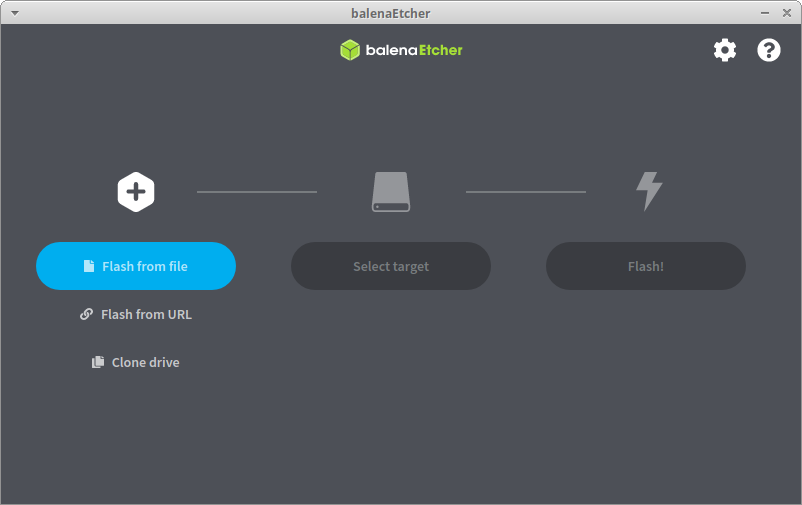
\includegraphics[width=0.9\linewidth,height=8cm,keepaspectratio]{img/p02-02-etcher-a.png} %CHKTEX 8
		\caption{Selección de imagen a grabar}
		\label{fig:write-image-linux-a} %CHKTEX 24
	\end{subfigure}%
	\begin{subfigure}[b]{0.5\linewidth}
		\centering
		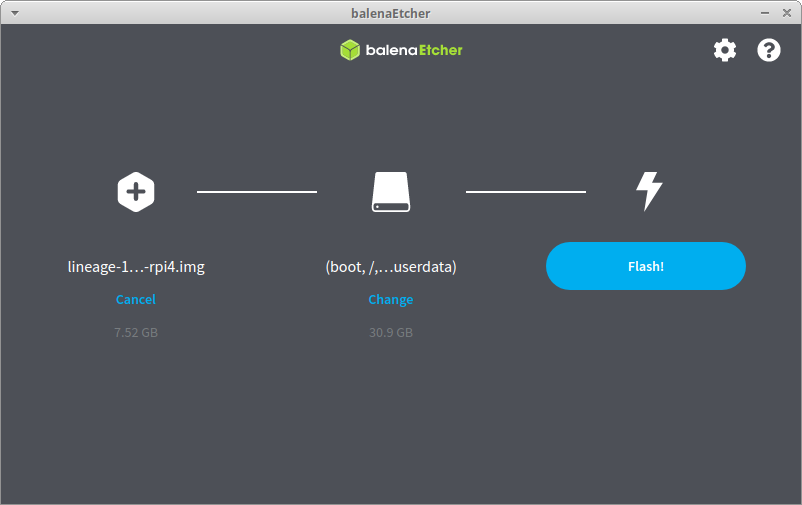
\includegraphics[width=0.9\linewidth,height=8cm,keepaspectratio]{img/p02-02-etcher-b.png} %CHKTEX 8
		\caption{Listo para grabar la imagen}
		\label{fig:write-image-linux-b} %CHKTEX 24
	\end{subfigure}
	\caption{Escritura de la imagen IMG de LineageOS en la microSD con Etcher}%
	\label{fig:write-image-linux} %CHKTEX 24
\end{figure}

Cuando la escritura de datos en la microSD termine, notará que ésta ha sido reparticionada con cuatro particiones:
\begin{itemize}[nosep]
	\item\texttt{boot} (circa.~128MiB) Partición de arranque tipo \textit{FAT32}.
	\item \texttt{/} (\emph{root}, circa.~1.5GiB) Partición raíz tipo \textit{EXT4} que contendrá el sistema base.
	\item \texttt{vendor} (circa.~256MiB) Partición para las aplicaciones del fabricante \textit{EXT4}.
	\item \texttt{userdata} (circa.~5.12GiB) Partición para las aplicaciones y datos del usuario \textit{EXT4}.
\end{itemize}

Finalmente, desmonte la tarjeta microSD e insértela en la Raspberry Pi.

\medskip{}

\begin{yellowbox}{Nota}
Si el sistema se reinicia antes de mostrar el asistente es debido a que el Kernel no es compatible con su modelo de Raspberry Pi. En ese caso, pruebe con otra versión o una más reciente.
\end{yellowbox}


% %% %%%%%%%%%%%%%%%%%%%%%%%%%%%%%%%%%%%%%%%%%%%%%%%%%%%%%%%%%%%%%%%%%%
%
% Step 4
%
% %% %%%%%%%%%%%%%%%%%%%%%%%%%%%%%%%%%%%%%%%%%%%%%%%%%%%%%%%%%%%%%%%%%%
% \clearpage
\subsection{Paso 4: Configurar LineageOS}%
Para configuar Raspbian, la Raspberry Pi deberá tener una tarjeta de memoria microSD con una imagen de LineageOS precargada y estar conectada a un monitor vía el puerto HDMI incorporado.
Además, se precisa de un teclado y apuntador (mouse) USB para realizar el proceso de configuración o, preferentemente, una pantalla táctil.
A continuación, conecte la Raspberry Pi y espere entre 1 y 3 minutos a que el sistema operativo cargue.

\begin{figure}[H]
	\centering
	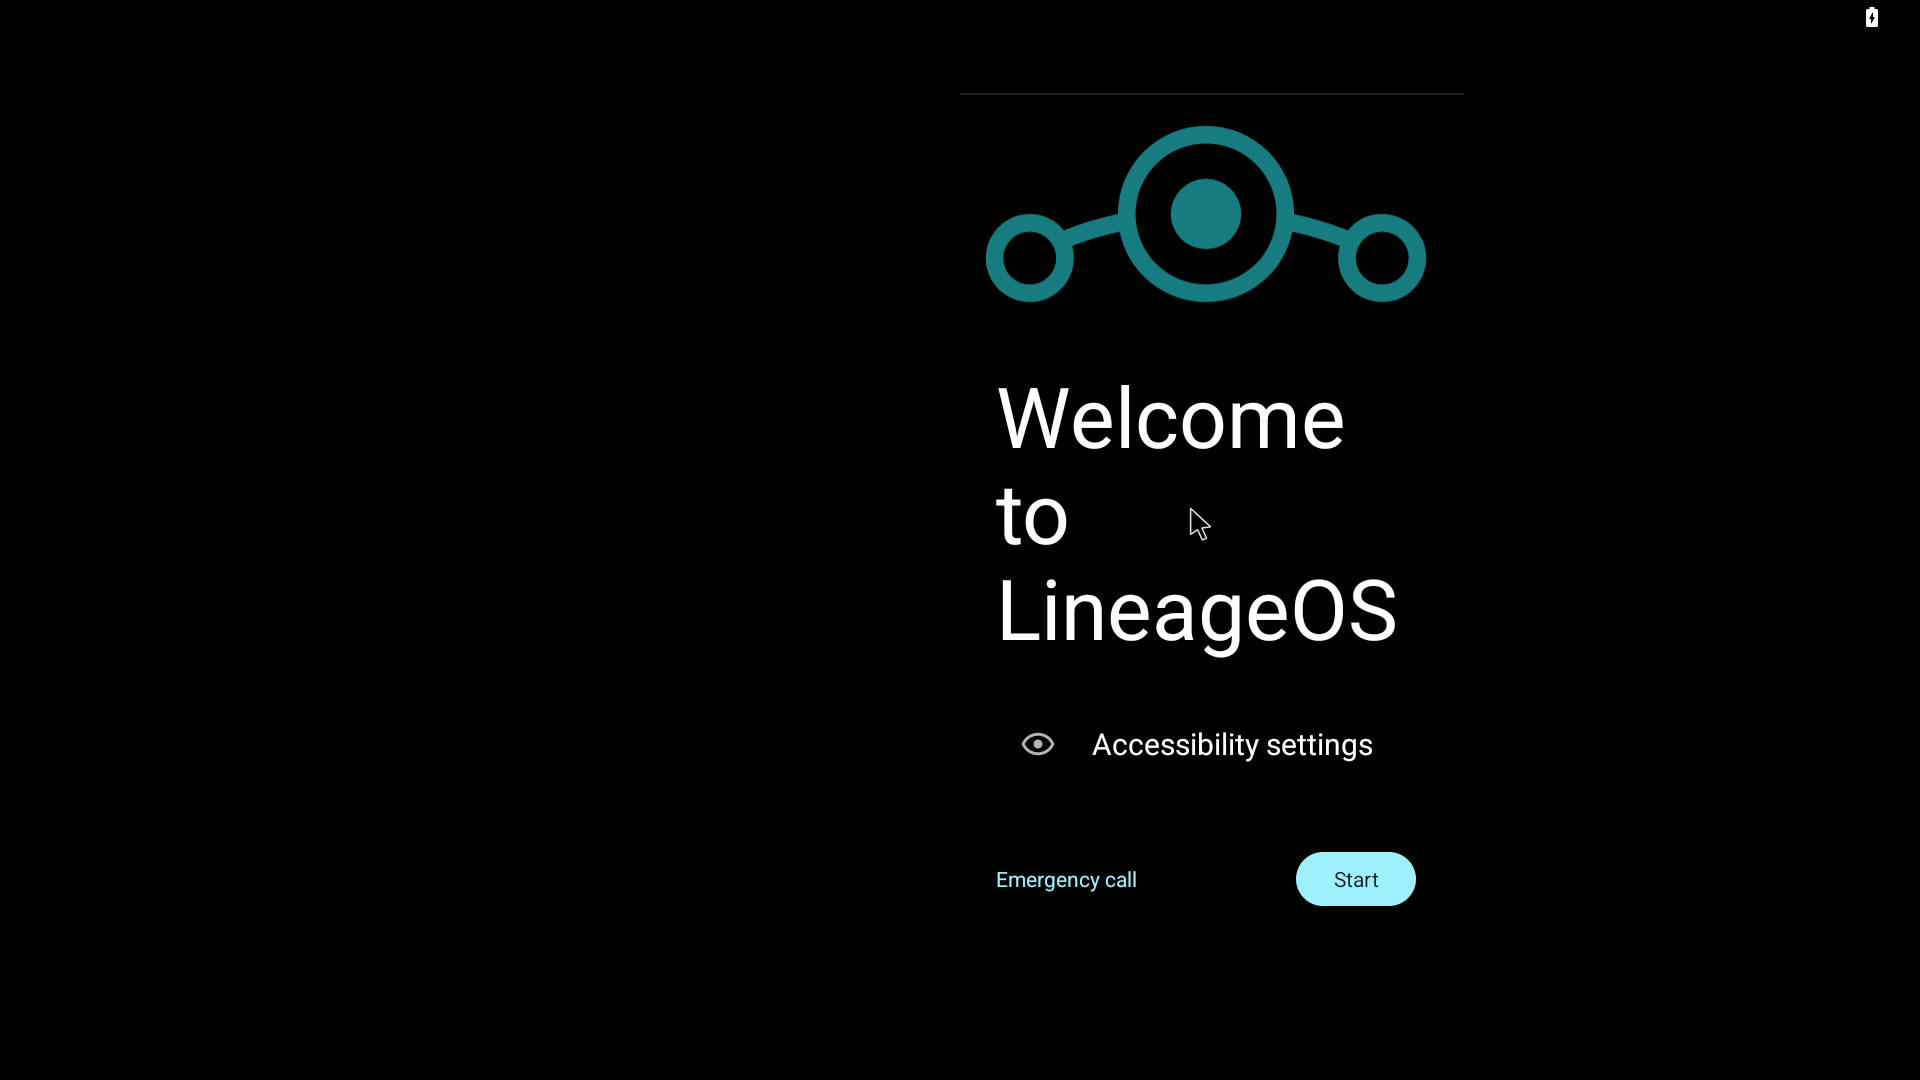
\includegraphics[width=0.9\linewidth,height=68mm,keepaspectratio]{img/p02-03-wizard-0.png} %CHKTEX 8
	\caption{Pantalla de inicio del asistente de configuración de LineageOS}
	\label{fig:lineageOS-wizard} %CHKTEX 24
\end{figure}

\noindent
Una vez terminado el proceso de arranque, siga el asistente como se muestra en la \Cref{fig:setup-wizard}.


\begin{figure}[H]
	\centering%
	\begin{subfigure}[b]{0.48\linewidth}
		\centering
		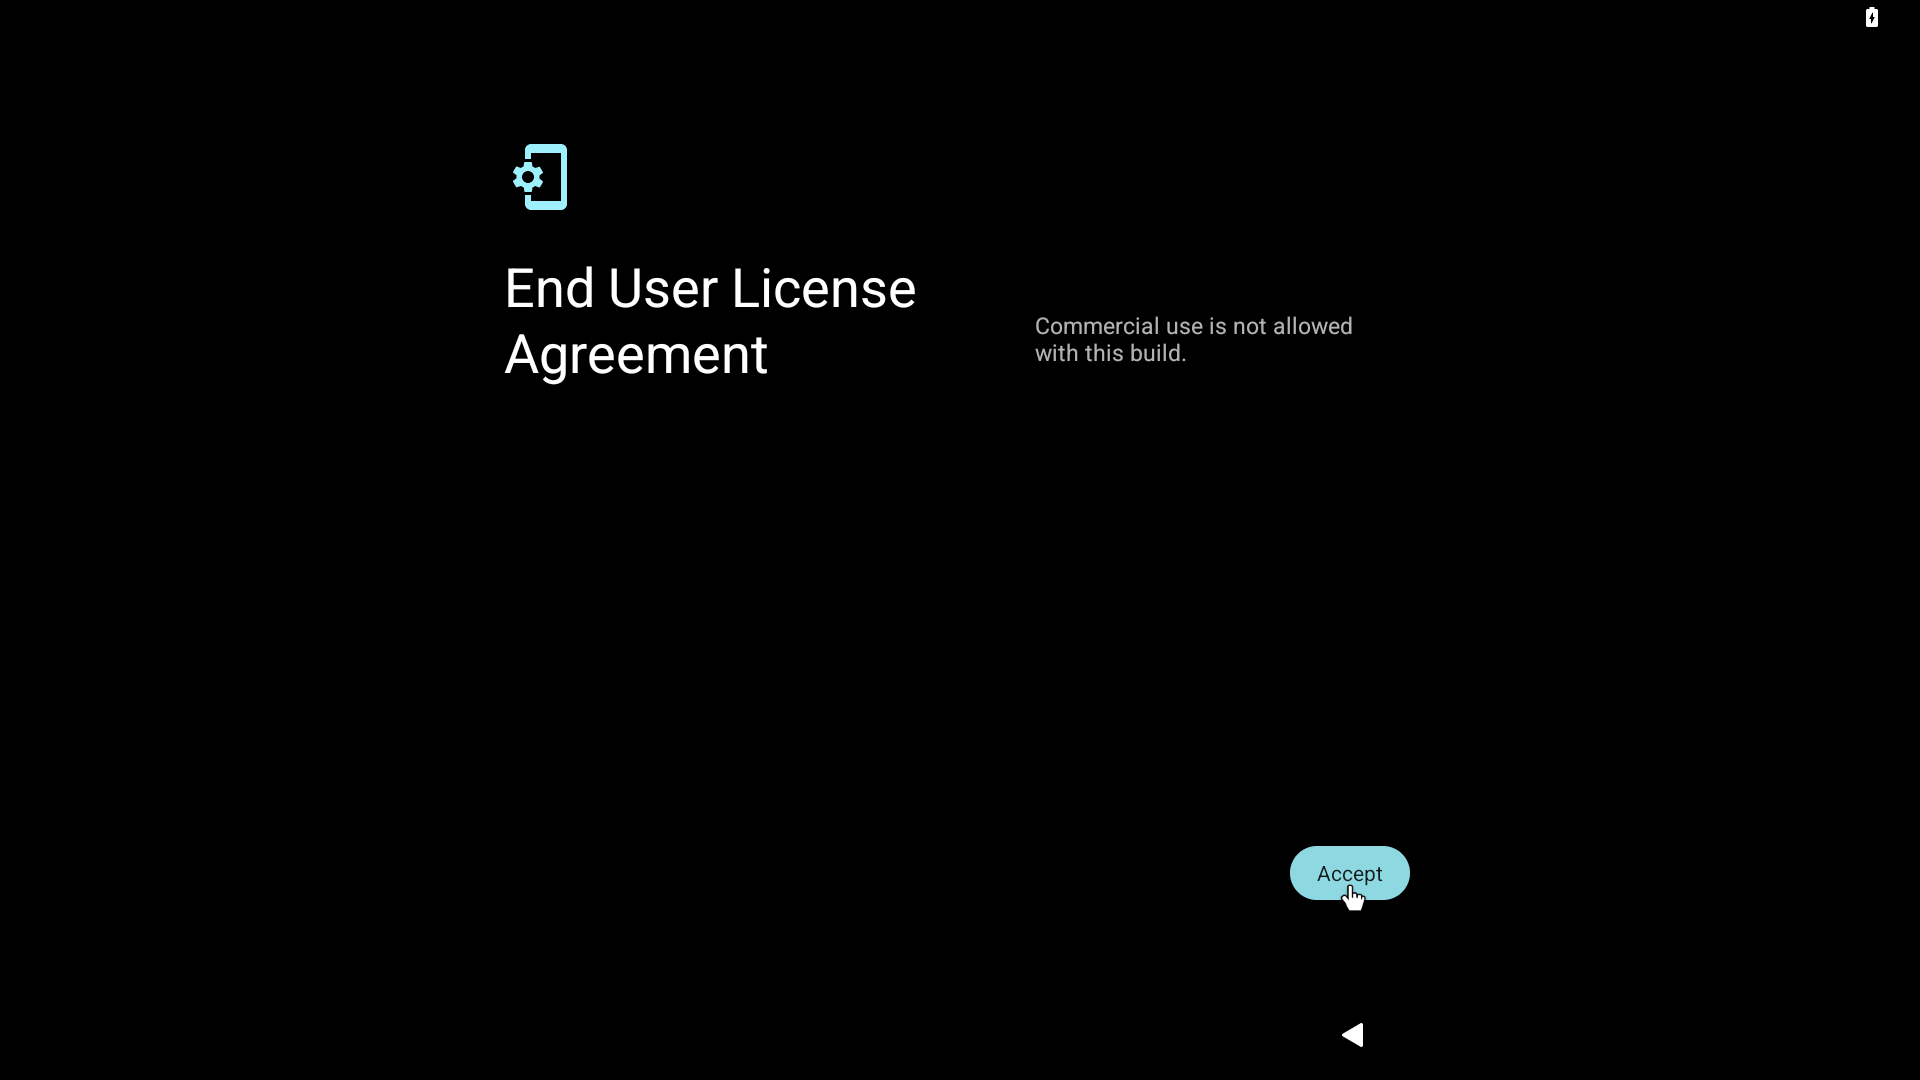
\includegraphics[width=0.9\linewidth,height=44mm,keepaspectratio]{img/p02-03-wizard-1.png} %CHKTEX 8
		\caption{Paso 1\\Acepte el acuerdo de licencia\\~}
		\label{fig:setup-wizard-step-1} %CHKTEX 24
	\end{subfigure}%
	\begin{subfigure}[b]{0.48\linewidth}
		\centering
		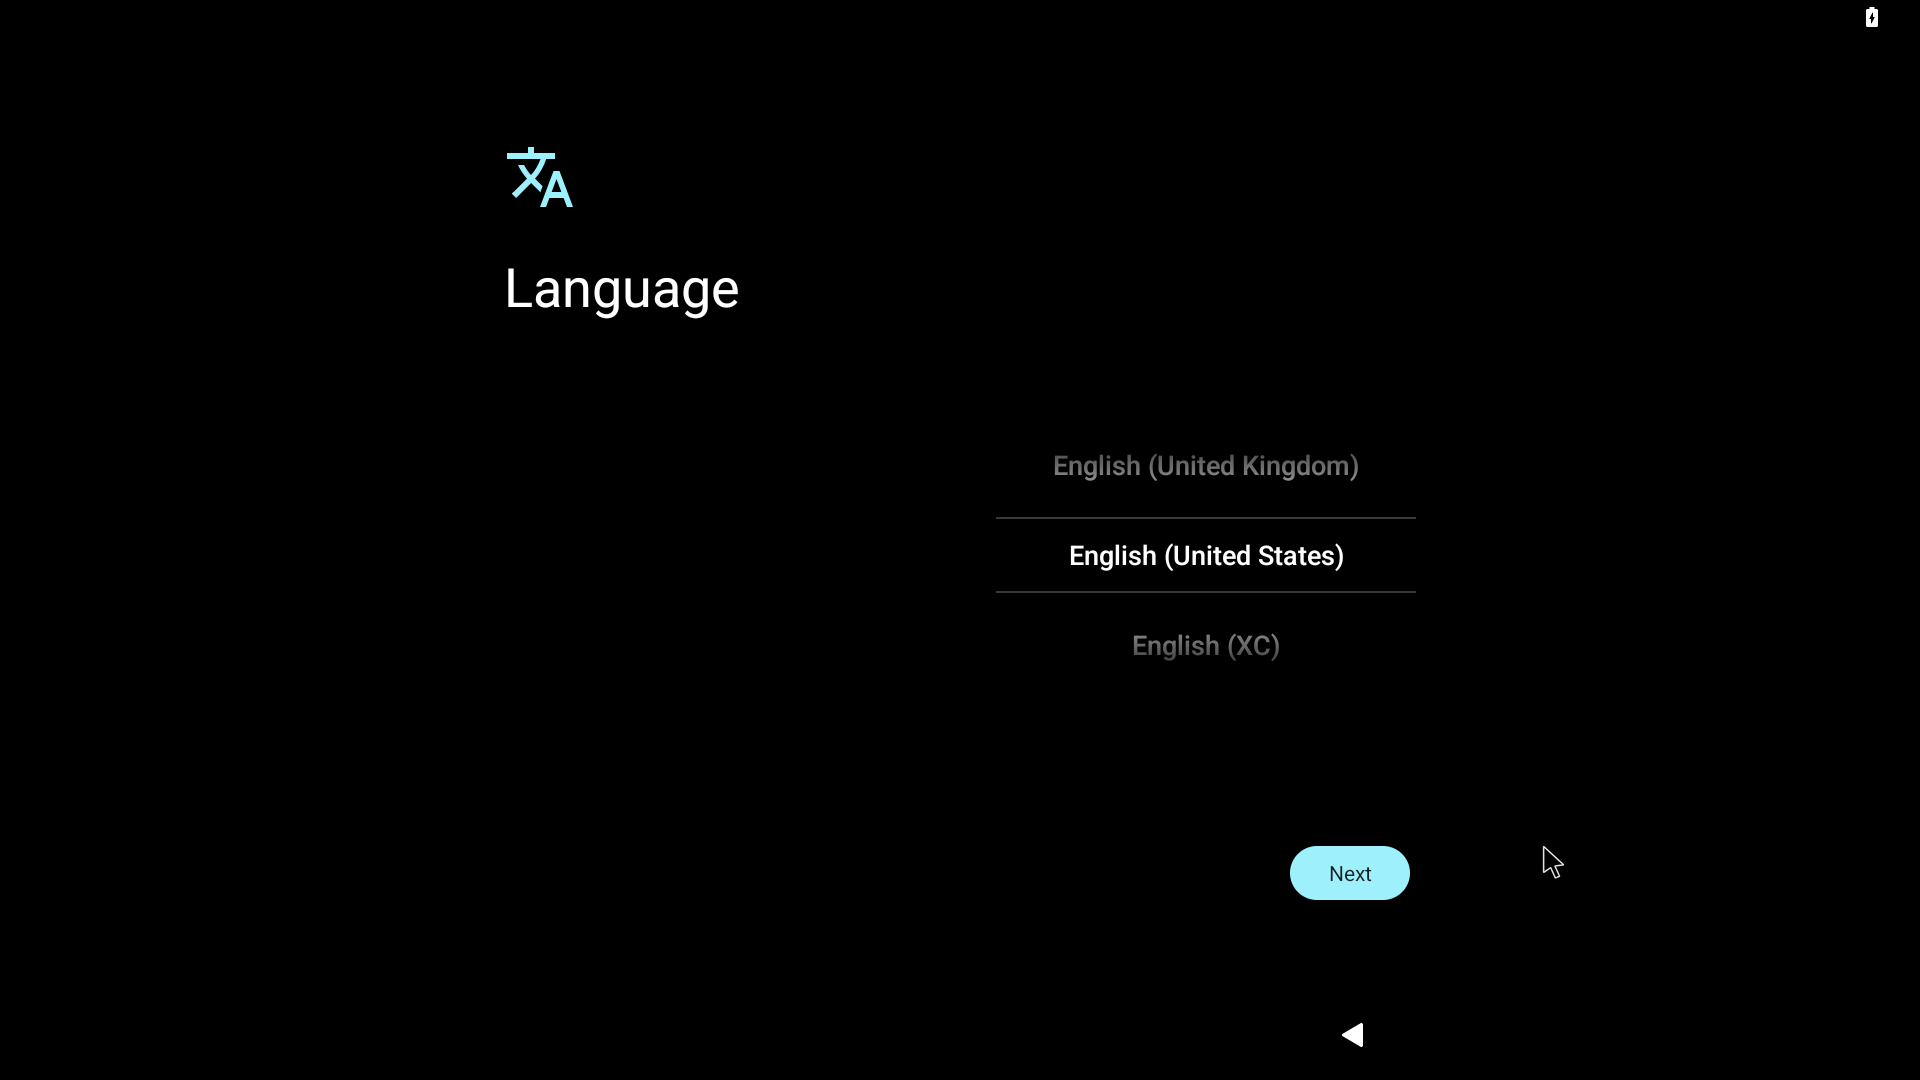
\includegraphics[width=0.9\linewidth,height=44mm,keepaspectratio]{img/p02-03-wizard-2.png} %CHKTEX 8
		\caption{Paso 2\\Seleccione el idioma\\~}
		\label{fig:setup-wizard-step-2} %CHKTEX 24
	\end{subfigure}\\
\end{figure}%
\begin{figure}[H]
	\ContinuedFloat%
	\centering%
	\begin{subfigure}[b]{0.48\linewidth}
		\centering
		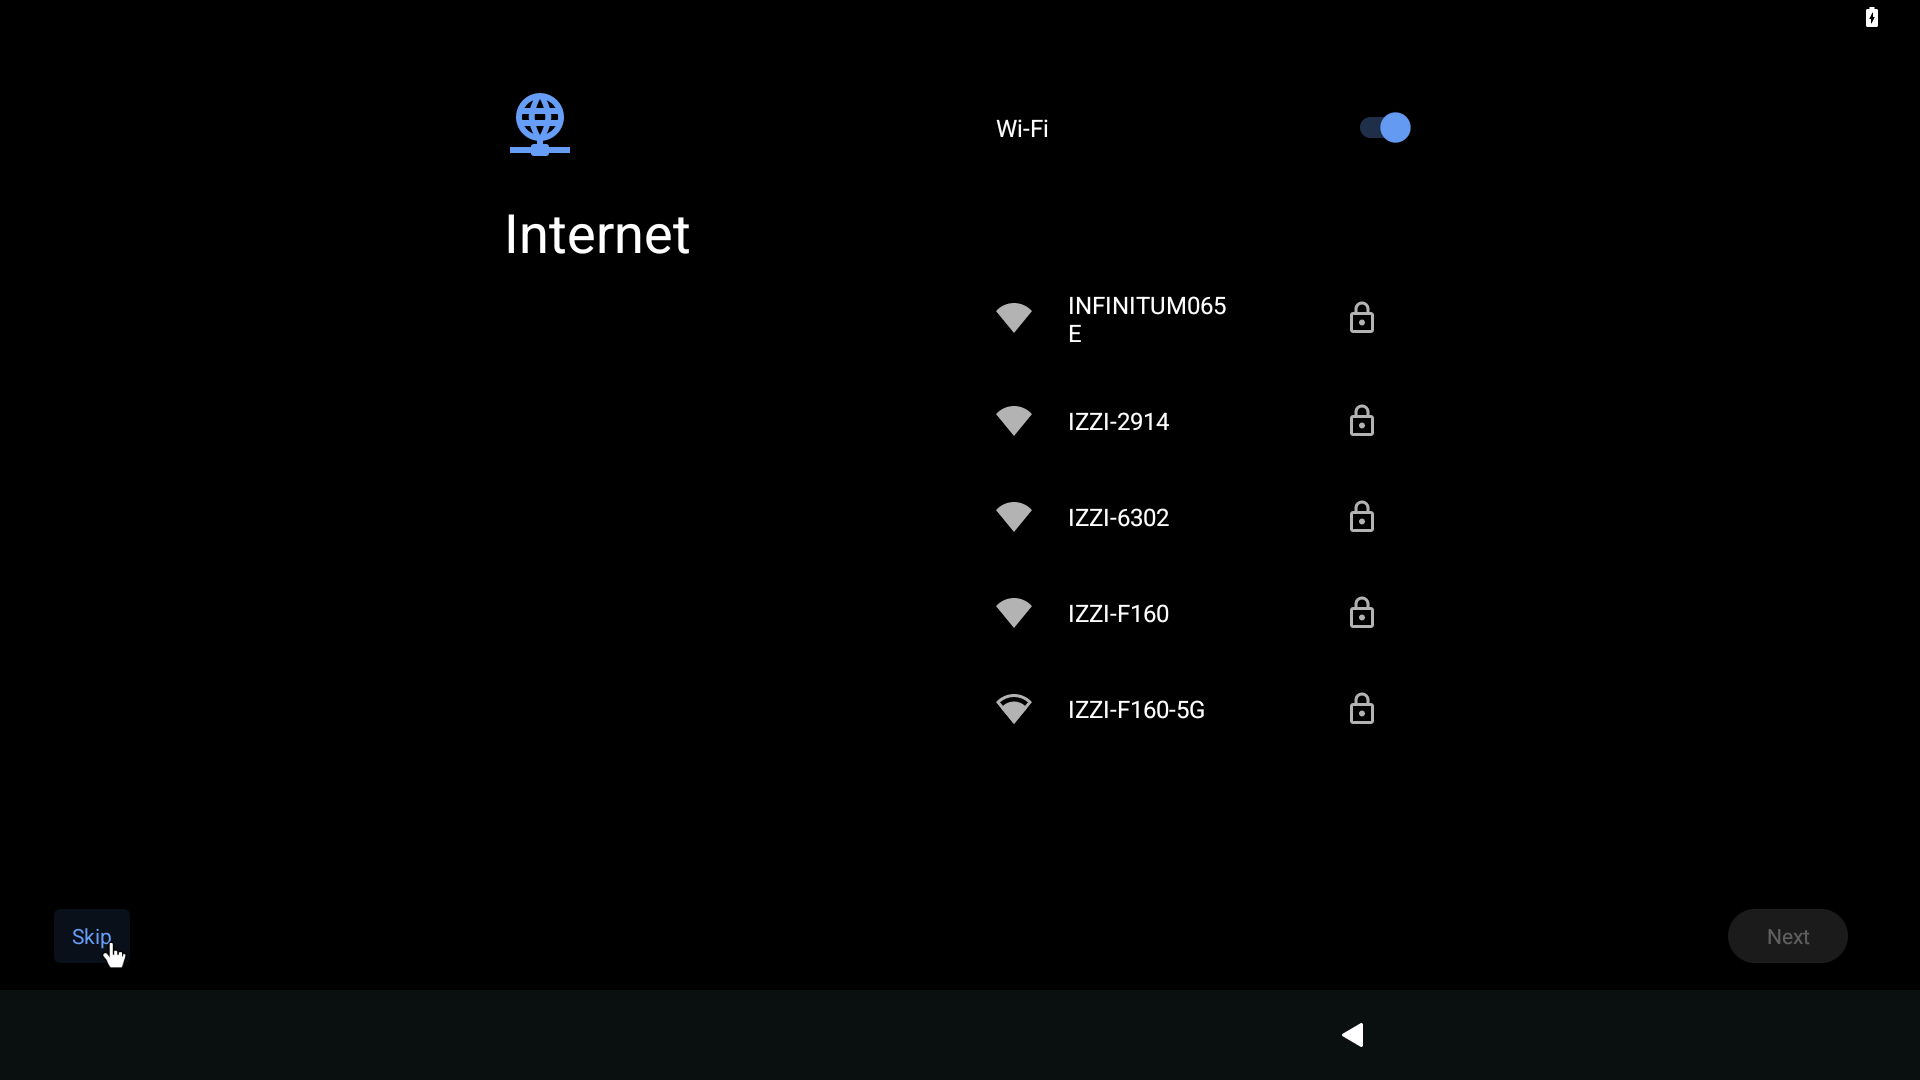
\includegraphics[width=0.9\linewidth,height=44mm,keepaspectratio]{img/p02-03-wizard-3.png} %CHKTEX 8
		\caption{Paso 3\\Omita la conexión a internet\\~}
		\label{fig:setup-wizard-step-3} %CHKTEX 24
	\end{subfigure}%
	\begin{subfigure}[b]{0.48\linewidth}
		\centering
		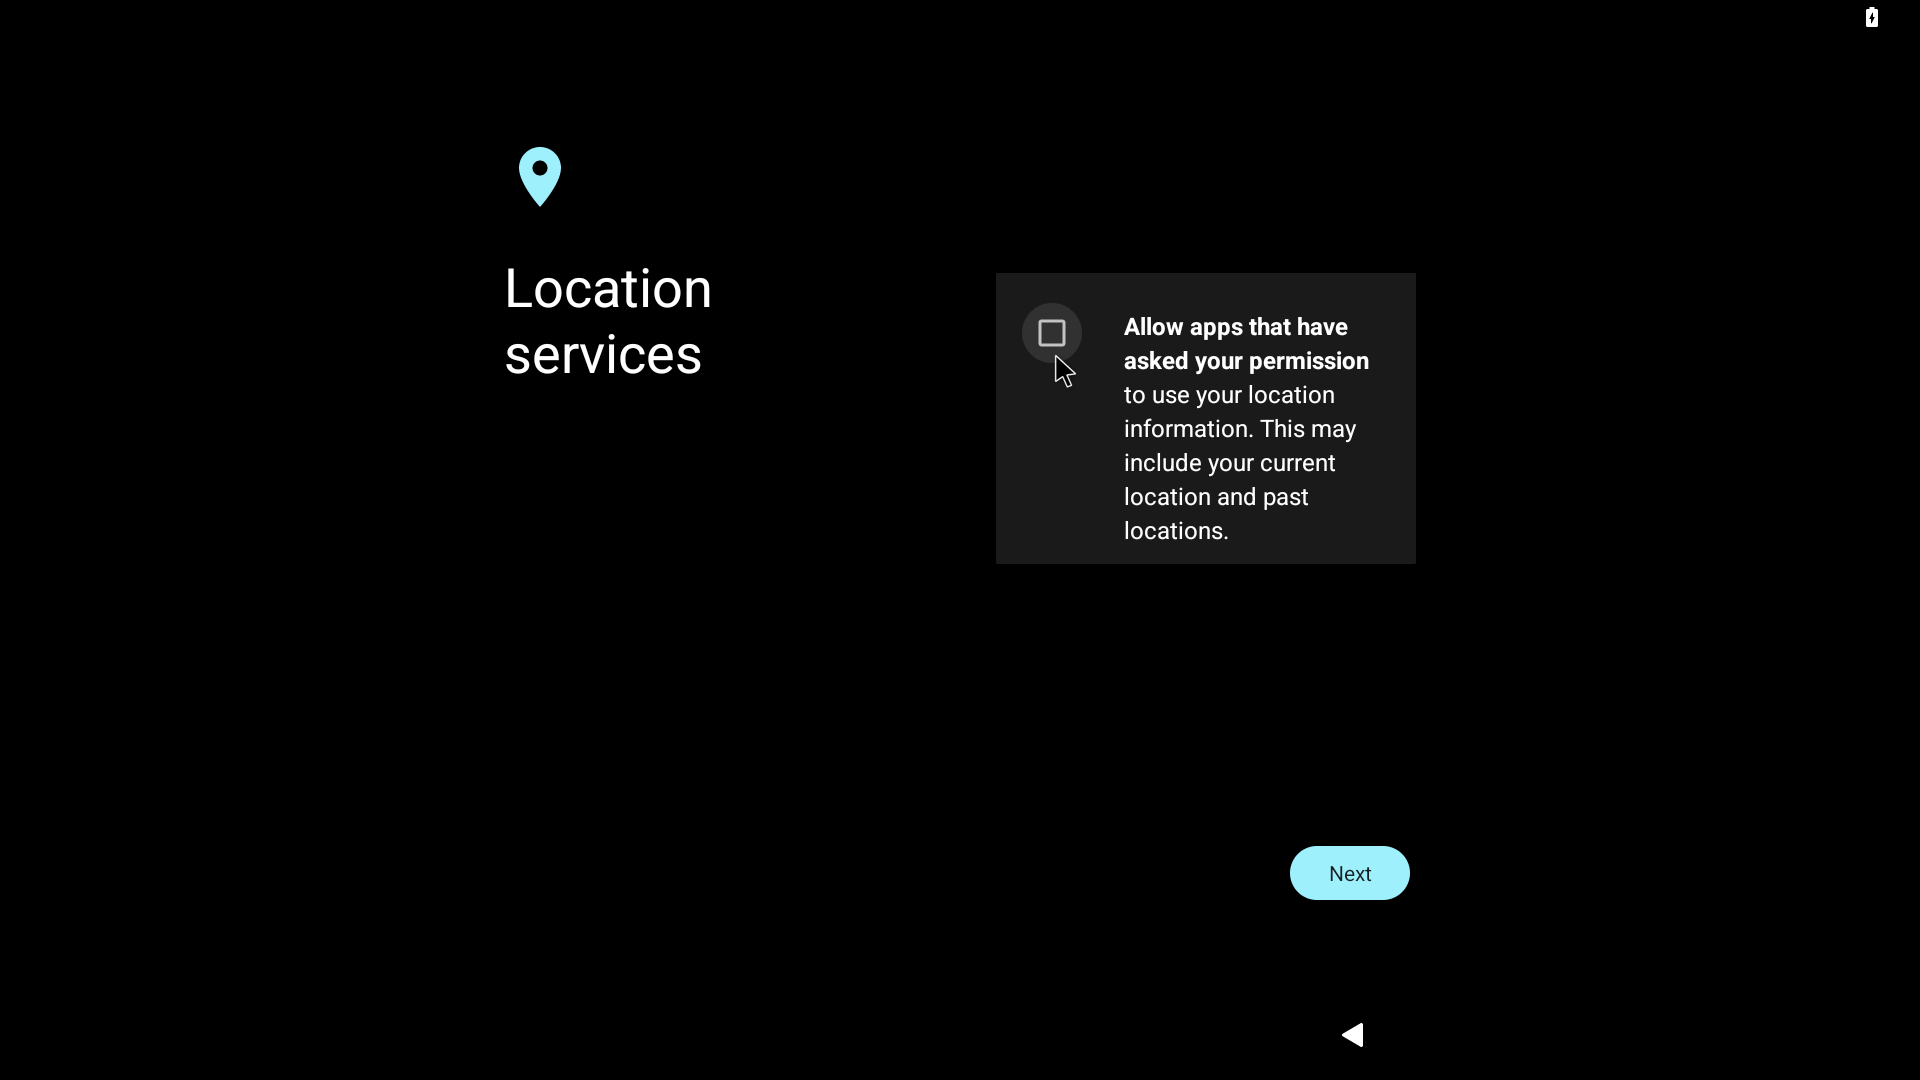
\includegraphics[width=0.9\linewidth,height=44mm,keepaspectratio]{img/p02-03-wizard-4.png} %CHKTEX 8
		\caption{Paso 4\\Deshabilite los servicios de localización\\~}
		\label{fig:setup-wizard-step-4} %CHKTEX 24
	\end{subfigure}\\
	\begin{subfigure}[b]{0.48\linewidth}
		\centering
		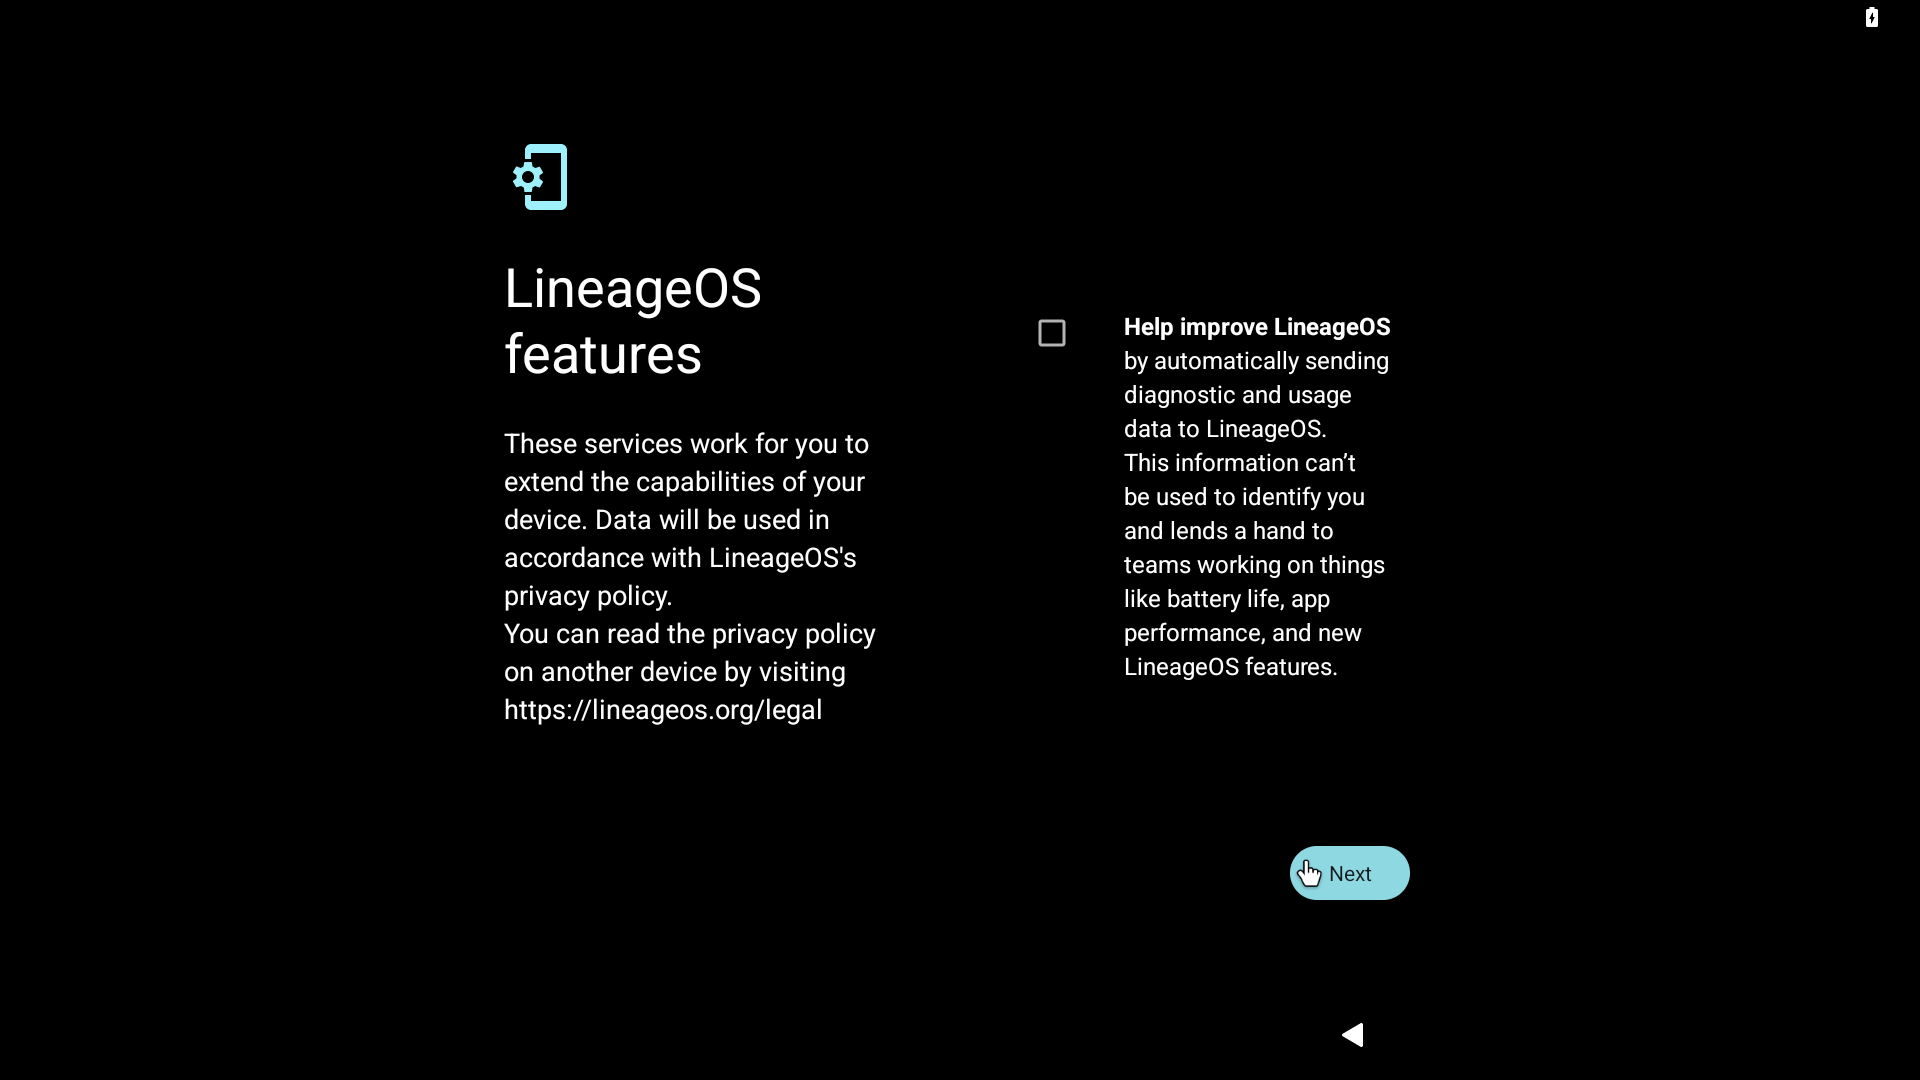
\includegraphics[width=0.9\linewidth,height=44mm,keepaspectratio]{img/p02-03-wizard-5.png} %CHKTEX 8
		\caption{Paso 5\\Desuscríbase del envío de datos diagnósticos\\~}
		\label{fig:setup-wizard-step-5} %CHKTEX 24
	\end{subfigure}%
	\begin{subfigure}[b]{0.48\linewidth}
		\centering
		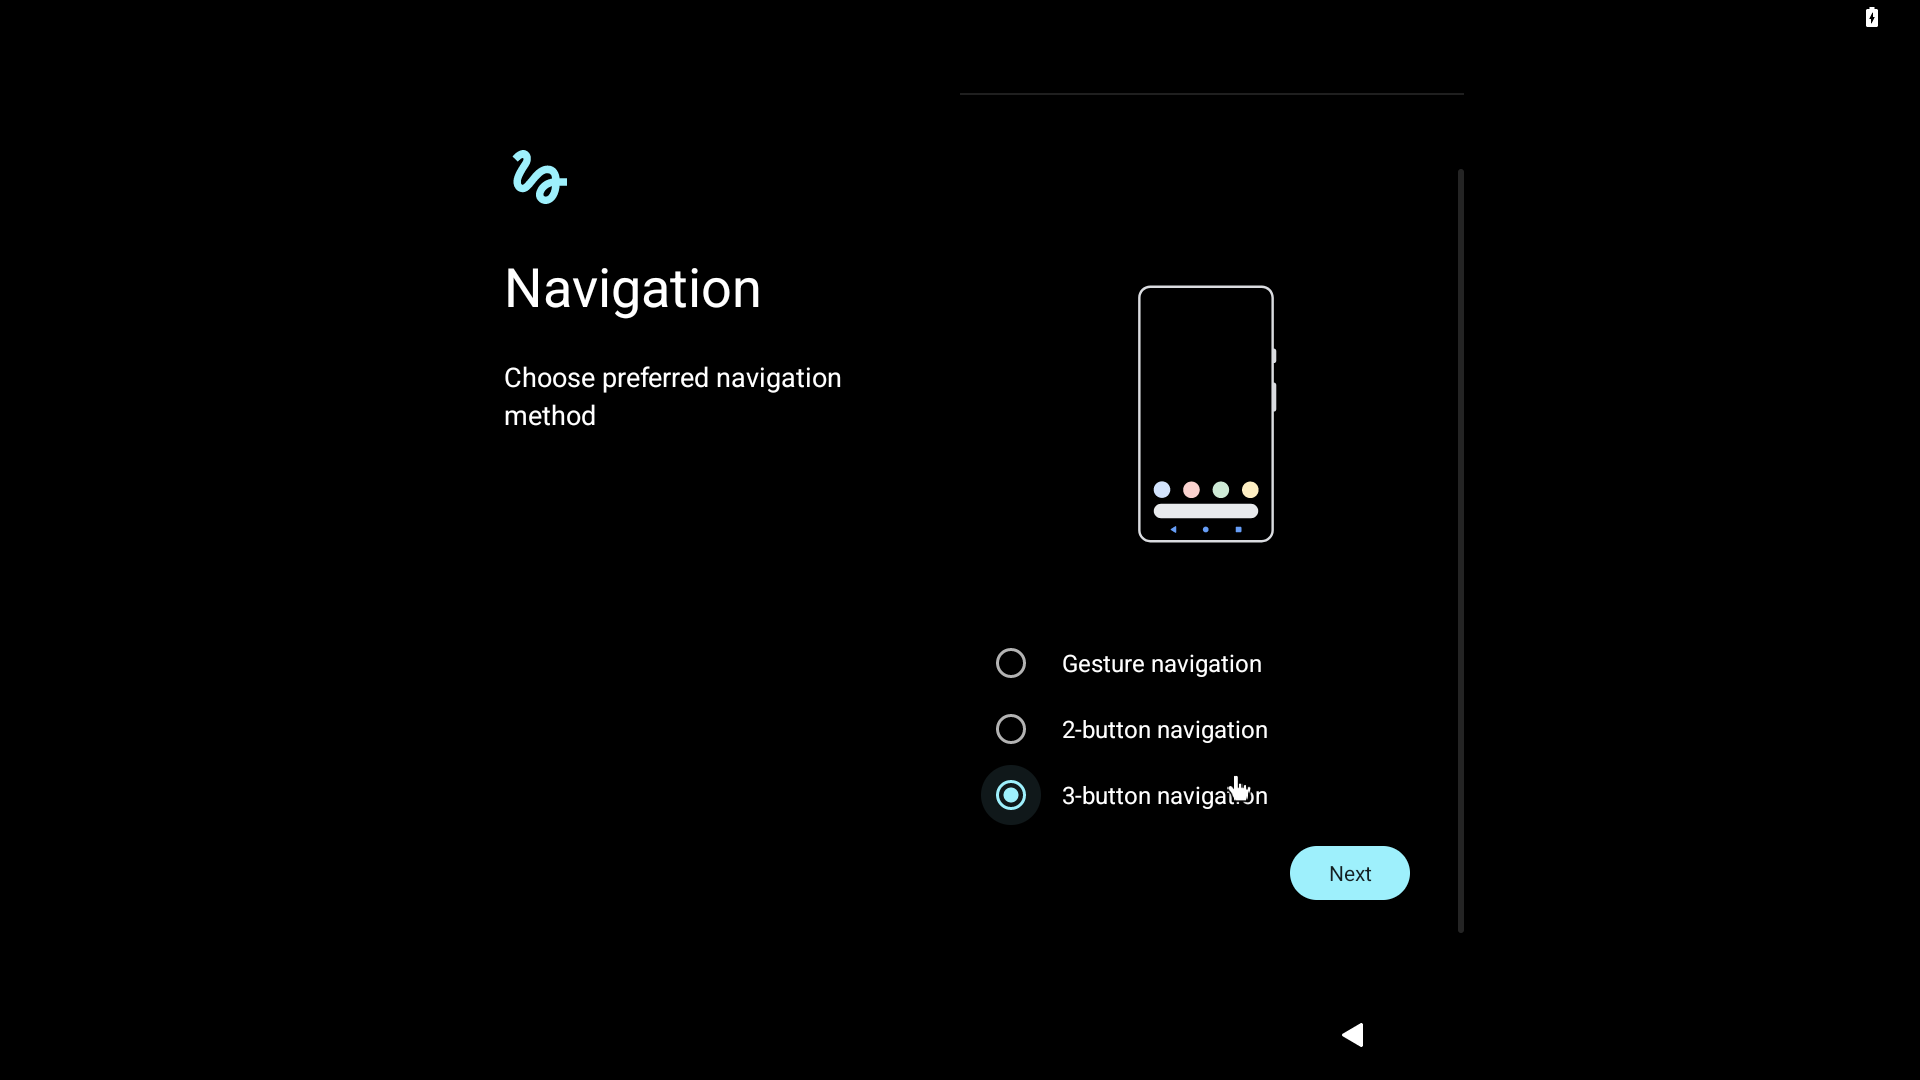
\includegraphics[width=0.9\linewidth,height=44mm,keepaspectratio]{img/p02-03-wizard-6.png} %CHKTEX 8
		\caption{Paso 6\\Elija los botones de navegación del sistema\\~}
		\label{fig:setup-wizard-step-6} %CHKTEX 24
	\end{subfigure}\\%
	\begin{subfigure}[b]{0.48\linewidth}
		\centering
		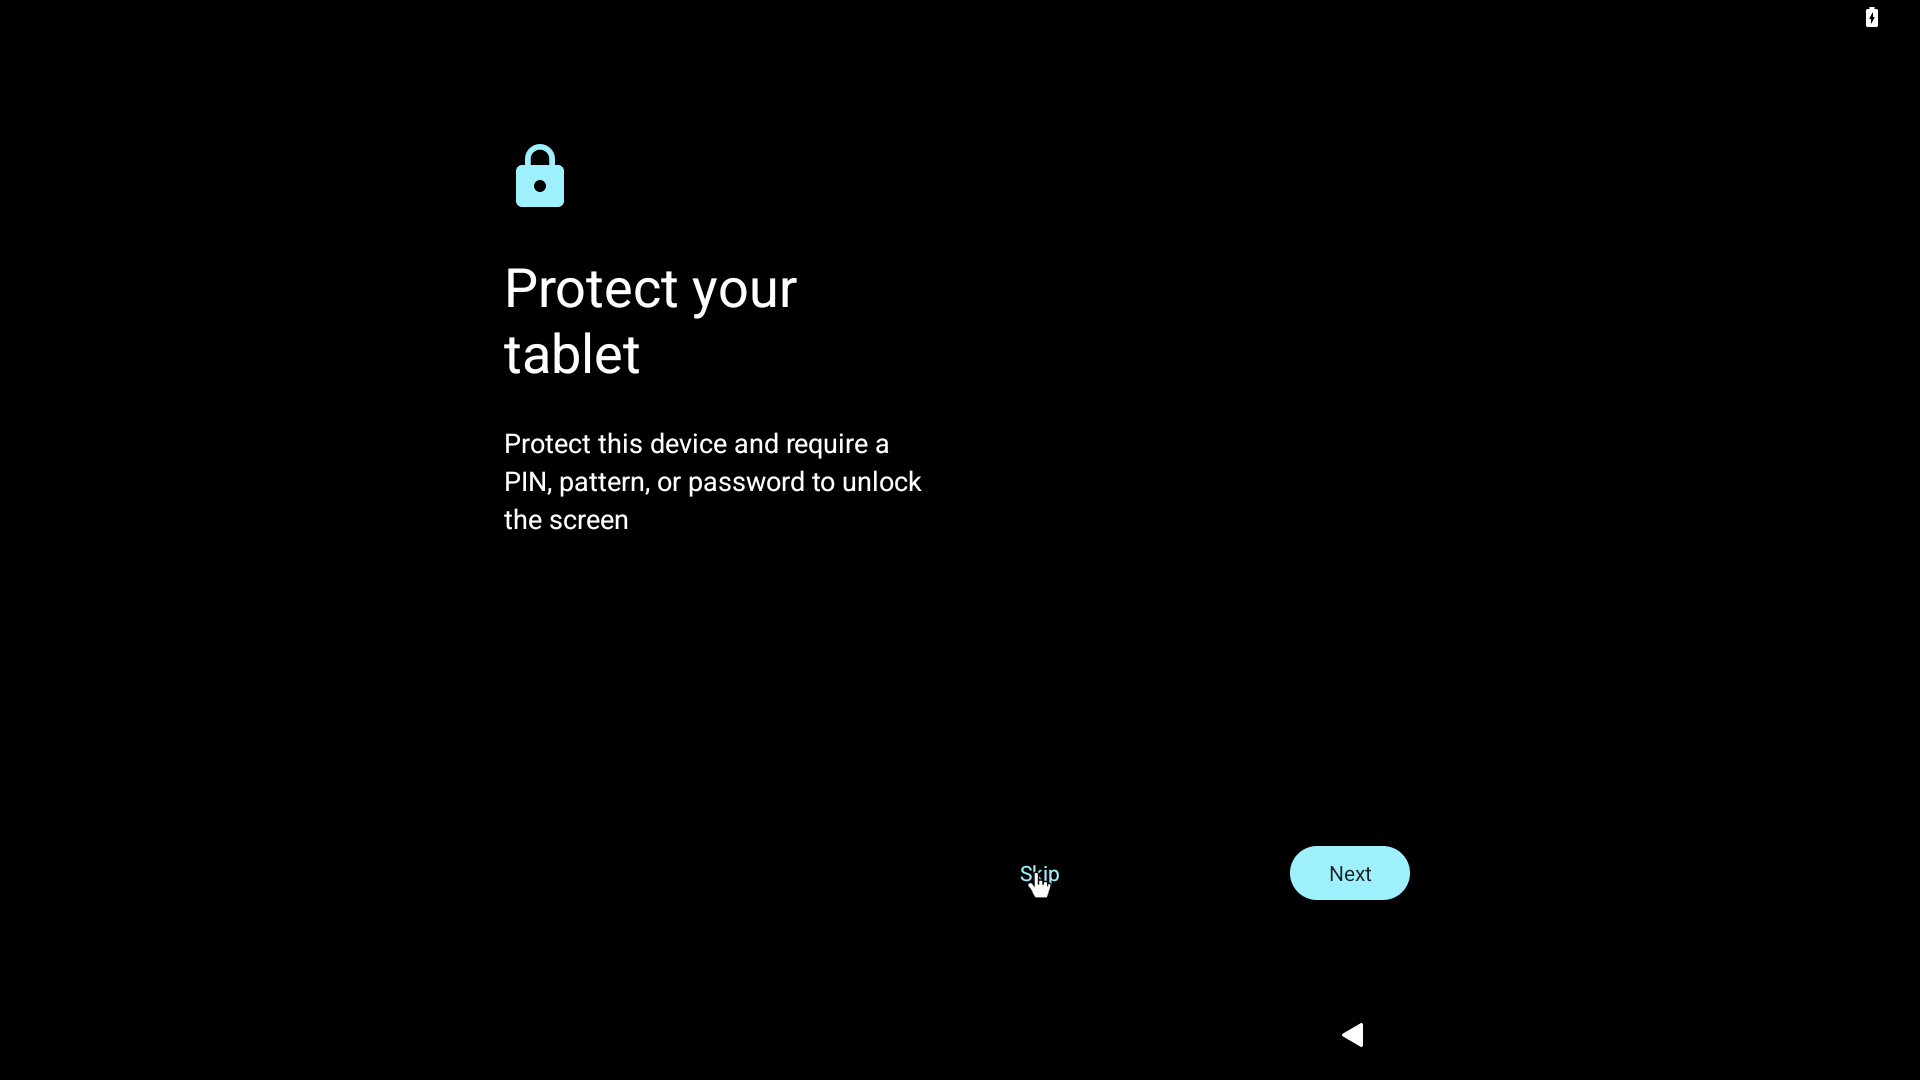
\includegraphics[width=0.9\linewidth,height=44mm,keepaspectratio]{img/p02-03-wizard-7.png} %CHKTEX 8
		\caption{Paso 7\\Omita la generación del PIN o contraseña\\~}
		\label{fig:setup-wizard-step-7} %CHKTEX 24
	\end{subfigure}%
	\begin{subfigure}[b]{0.48\linewidth}
		\centering
		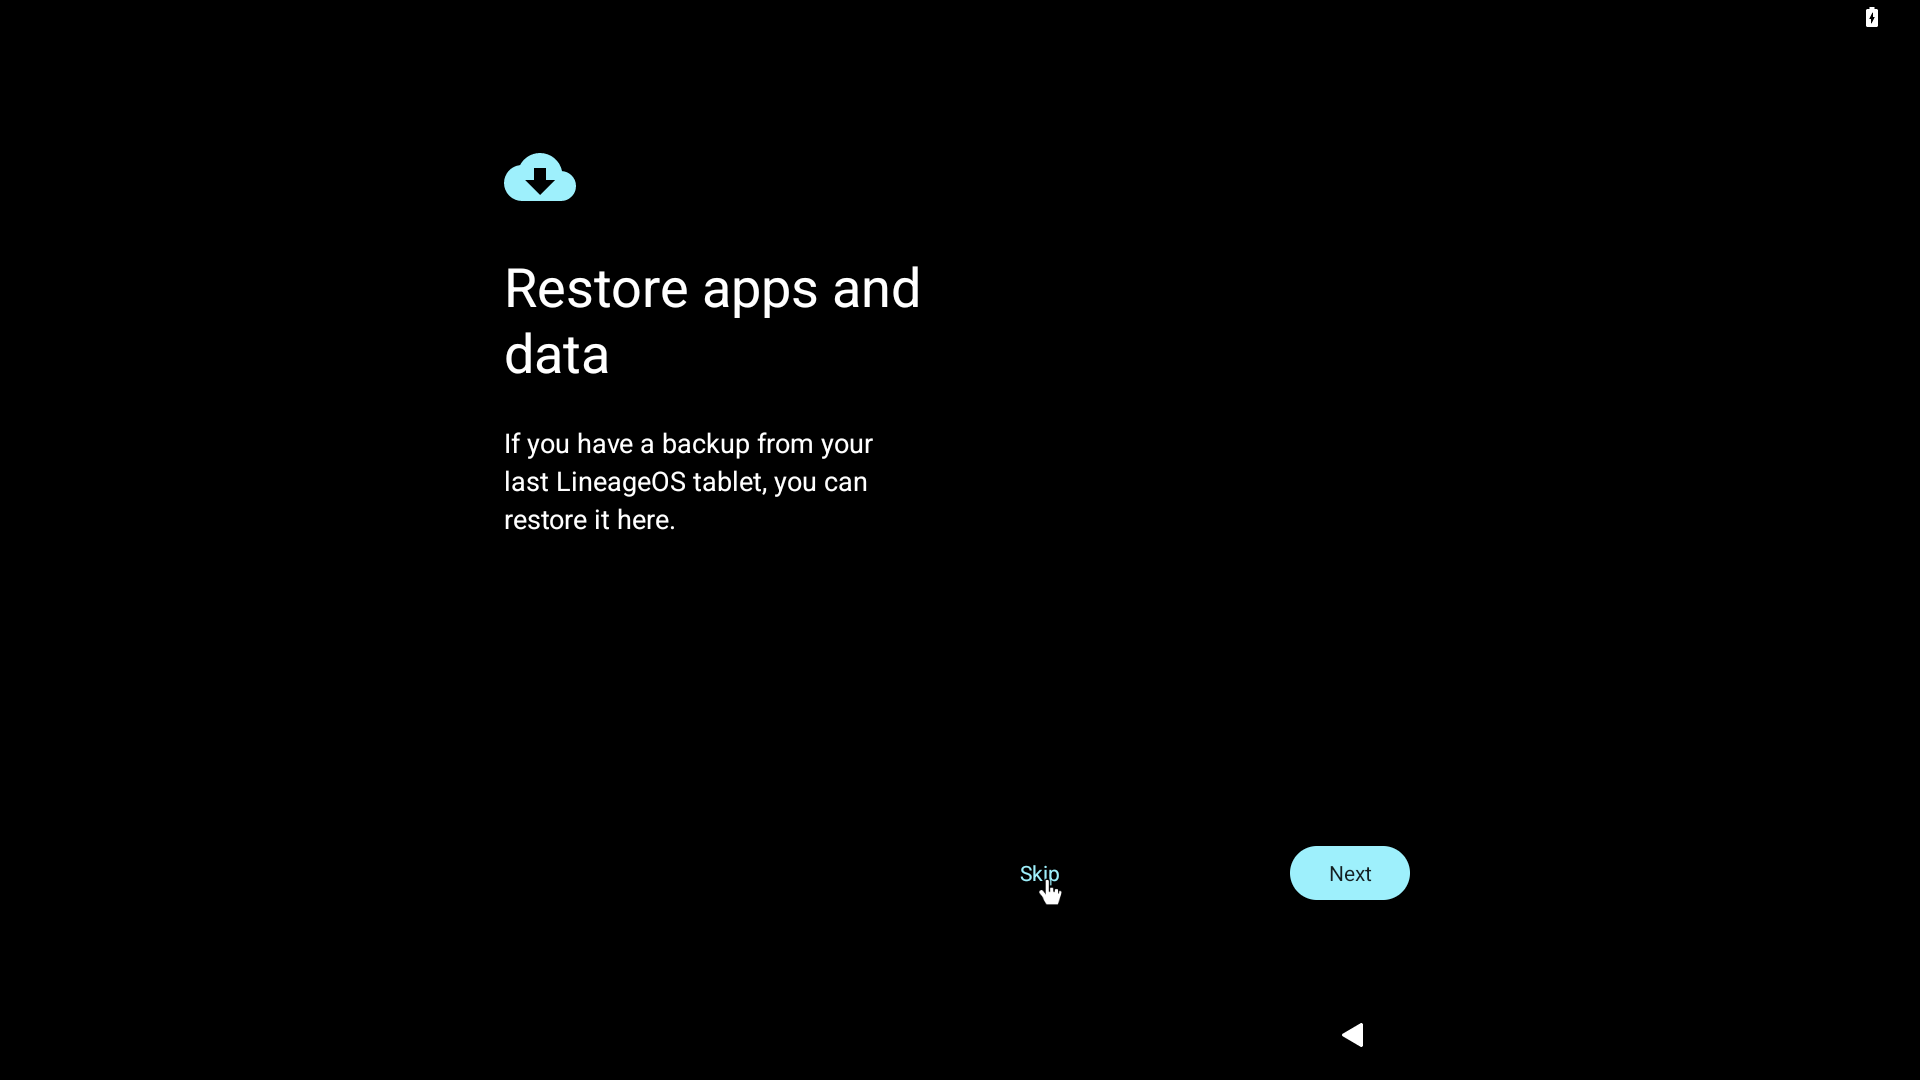
\includegraphics[width=0.9\linewidth,height=44mm,keepaspectratio]{img/p02-03-wizard-8.png} %CHKTEX 8
		\caption{Paso 8\\Omita la sincronización con la nube\\~}
		\label{fig:setup-wizard-step-8} %CHKTEX 24
	\end{subfigure}\\
	\caption{Asistente de configuración de LineageOS}%
	\label{fig:setup-wizard} %CHKTEX 24
\end{figure}

\medskip{}
\begin{greenbox}{Nota}
Algunos modelos de Raspberry Pi podrían no detectar correctamente la resolución del monitor, causando que la pantalla esté desajustada.
\medskip{}
Si esto sucediere, utilice las flechas del teclado para seleccionar el boton \emph{Start} en la primer pantalla.
A partir de este punto, los botones deberían ser visibles sin mayores complicaciones.
Al terminar el asistente podrá ajustar la pantalla en las opciones de Android.
\end{greenbox}
\medskip{}

\noindent
Una vez concluido el asistente de configuración, de click en siguiente para comenzar a usar su sistema Android en la Raspberry Pi (véase~\Cref{fig:setup-wizard-end,fig:lineageOS-desktop}).
\begin{figure}[H]
	\centering
	
\includegraphics[width=0.9\linewidth,height=68mm,keepaspectratio]{img/p02-03-wizard-9.png} %CHKTEX 8
	\caption{Fin del asistente de configuración de LineageOS}
	\label{fig:lineageOS-wizard-end} %CHKTEX 24
\end{figure}

Ahora observará el escritorio de Android Lineage OS en su Rasberyy Pi.

\begin{figure}[H]
	\centering
	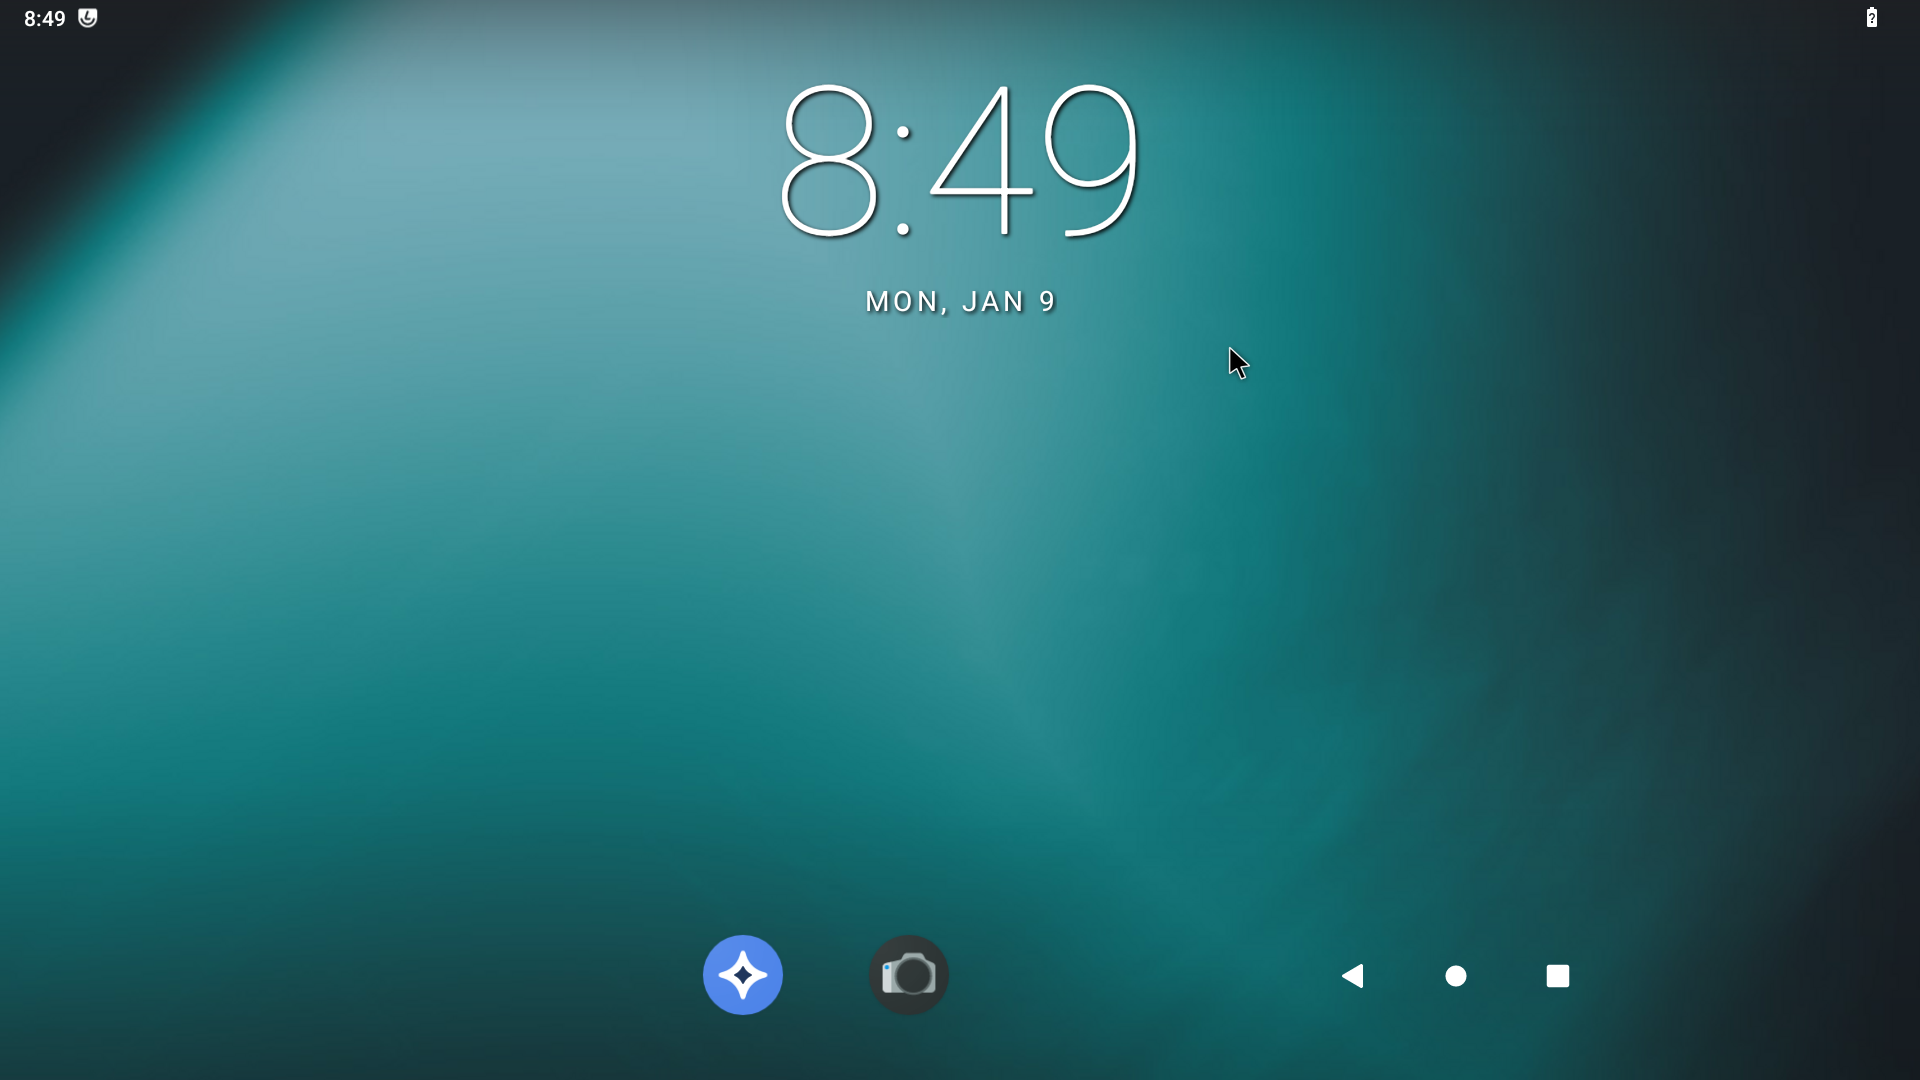
\includegraphics[width=0.9\linewidth,height=68mm,keepaspectratio]{img/P02-04-desktop.png} %CHKTEX 8
	\caption{Escritorio de LineageOS}
	\label{fig:lineageOS-desktop} %CHKTEX 24
\end{figure}

% %% %%%%%%%%%%%%%%%%%%%%%%%%%%%%%%%%%%%%%%%%%%%%%%%%%%%%%%%%%%%%%%%%%%
%
% Step 5
%
% %% %%%%%%%%%%%%%%%%%%%%%%%%%%%%%%%%%%%%%%%%%%%%%%%%%%%%%%%%%%%%%%%%%%
% \clearpage
\subsection{Paso 5: Instalación de \emph{Google Play}}%
\begin{yellowbox}{Nota}
Para completar este paso necesitará una conexión a internet.
\end{yellowbox}
\medskip{}

Este paso es el más complicado de toda la instalación, principalmente porque no es posible utilizar la tienda oficial \emph{Google Play} de Android ya que la Raspberry Pi no se considera un dispositivo comercializable con Android licenciable.
Por este motivo, es necesario instalar una tienda alternativa siguiendo una seire de sencillos pasos.

\begin{enumerate}
	\item Abra la aplicación \emph{Settings} (Configuración).
	\item Vaya a \emph{System} (Sistema).
	\item Vaya a \emph{Advanced settings} (Configuraciones avanzadas).
	\item Habilite la primera opción \emph{Reboot to recovery} (Reinicio de recuperación).
\end{enumerate}

\begin{figure}[H]
	\centering
	\begin{subfigure}{\linewidth}
		\centering
		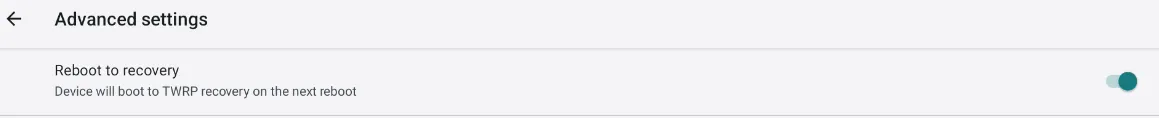
\includegraphics[width=0.9\linewidth,height=68mm,keepaspectratio]{img/p02-05-recovery-boot.png} %CHKTEX 8
		\caption{Opción \emph{Reboot to recovery} habilitada}%
		\label{fig:recovery-boot} %CHKTEX 24
	\end{subfigure}\\%
	\begin{subfigure}{\linewidth}
		\centering
		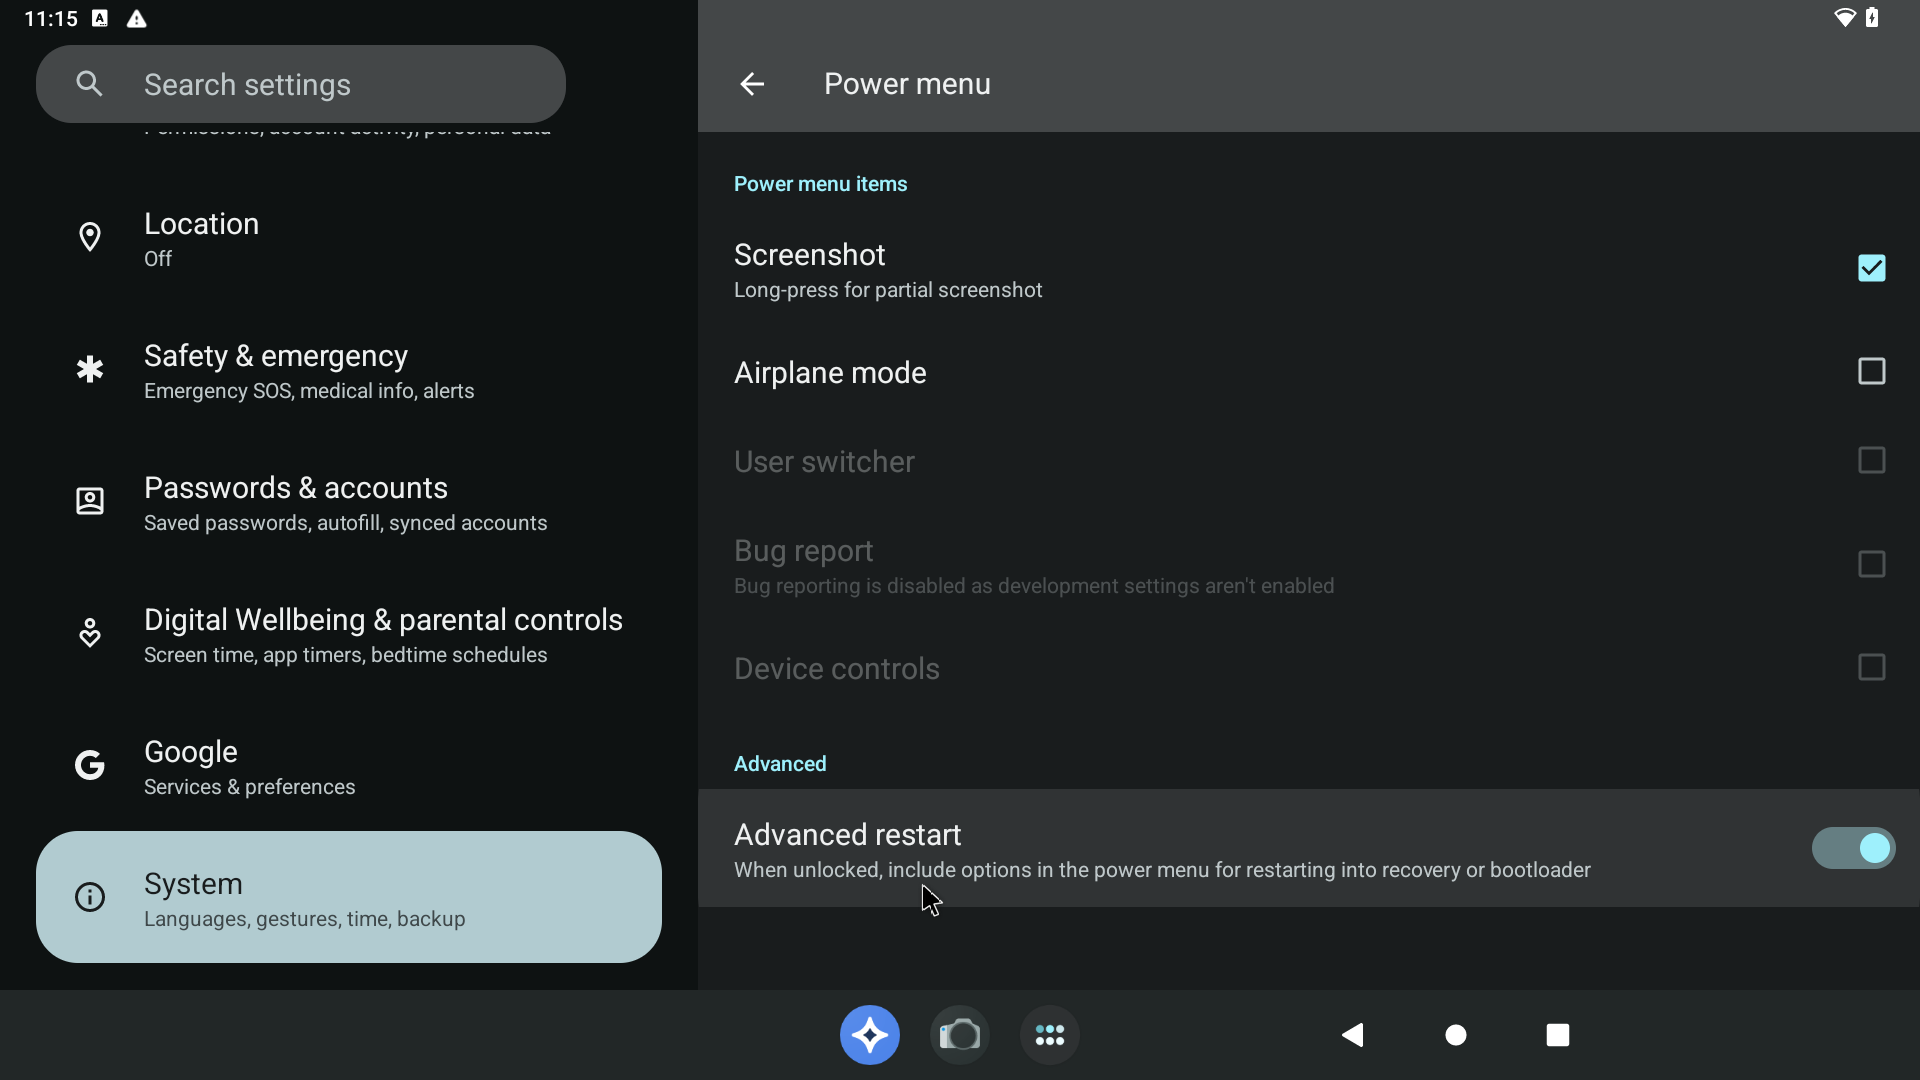
\includegraphics[width=0.9\linewidth,height=68mm,keepaspectratio]{img/p02-05-advanced-restart.png} %CHKTEX 8
		\caption{Opción \emph{Advanced Restart} habilitada}%
		\label{fig:advanced-restart} %CHKTEX 24
	\end{subfigure}
	\caption{Activación de reinicio de recuperación}%
	\label{fig:recovery-restart} %CHKTEX 24
\end{figure}

\medskip{}
\begin{greenbox}{Nota}
La ubicación de la opción \emph{Reboot to recovery} puede cambiar entre versiones.
Si no la encuentra en \emph{Settings} \(\rightarrow{}\) \emph{System} \(\rightarrow{}\) \emph{Advanced settings}, búsquela en las configuraciones.
Por ejemplo en la versión 13 se encuentra en \emph{System}, \emph\emph{Buttons}, \emph{Power Menu}, \emph{Advanced Restart}.
\end{greenbox}
\medskip{}

A continuación de click en el botón de la batería para mostrar las opciones del dispositivo.
Seleccione \emph{Restart} (Reiniciar) y después \emph{Reccovery} (Recuperación).

\begin{figure}[H]
	\centering
	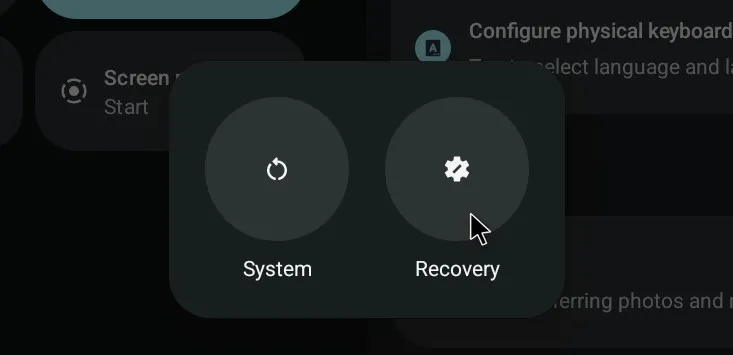
\includegraphics[width=0.9\linewidth,height=68mm,keepaspectratio]{img/p02-05-recovery-restart.png} %CHKTEX 8
	\caption{Opción \emph{Reboot to recovery} habilitada}
	\label{fig:recovery-restart} %CHKTEX 24
\end{figure}

Tras seleccionar esta opción, inserte la USB con y espere a que la Raspberry termine de cargar LineageOS. %CHKTEX 13
La pantalla será diferente esta vez pues se habrá iniciado en modo recuperación, algo parecido a como muestra la \Cref{fig:recovery-mode}.
Siga los siguientes pasos:

\begin{enumerate}
	\item De click en \emph{Mount} (Montar), opción desde donde puede montar una partición en específico.
	\item Busuqe su memoria USB en la lista de dispositivos montables y seleccione la partición pertinente (normalmente las memorias USB sólo tienen una partición).
	\item De regreso en la pantalla principal, de click en \emph{Install} (Instalar).
	\item De click en \emph{Select Storage} (Seleccionar Almacenamiento).
	\item Seleccione la unidad USB que acaba de montar.
	\item Cuando aparezcan los archivos almacenados en la unidad USB, de click en \emph{NikGapps} para instalarlo.
	\item Confirme que desea instalar \emph{NikGapps} deslizando a la derecha la barra de desplazamiento (véase~\Cref{fig:nikgapps-install-confirm}).
	\item Si la instalación se concluye con éxito, regresará a la pantalla principal.
	\item De click en \emph{Reboot} (Reiniciar).
	\item Elija \emph{System} (Sistema) para regresar al modo normal.
\end{enumerate}

\medskip{}
\begin{greenbox}{Nota}
	No seleccione la opción \emph{Reboot after installation is complete} (reiniciar al completar la instalación), ya que el sistema volvería  a arrancar en modo de recuperación automáticamente.
\end{greenbox}
\medskip{}

Cuando reinicie la Raspberry, busque la Play Store entre las aplicaciones (véase \Cref{fig:playstore}) e inicie sesión con su cuenta de Google.
Si la aplicación aparece haberse atascado, siga esperando hasta que se reciba respuesta del servidor.
Una vez que haya iniciado sesión, reinicie el dispositivo.

Ya puede instalar aplicaciones normalmente.

\begin{figure}[H]
	\centering%
	\begin{subfigure}[b]{0.5\linewidth}
		\centering
		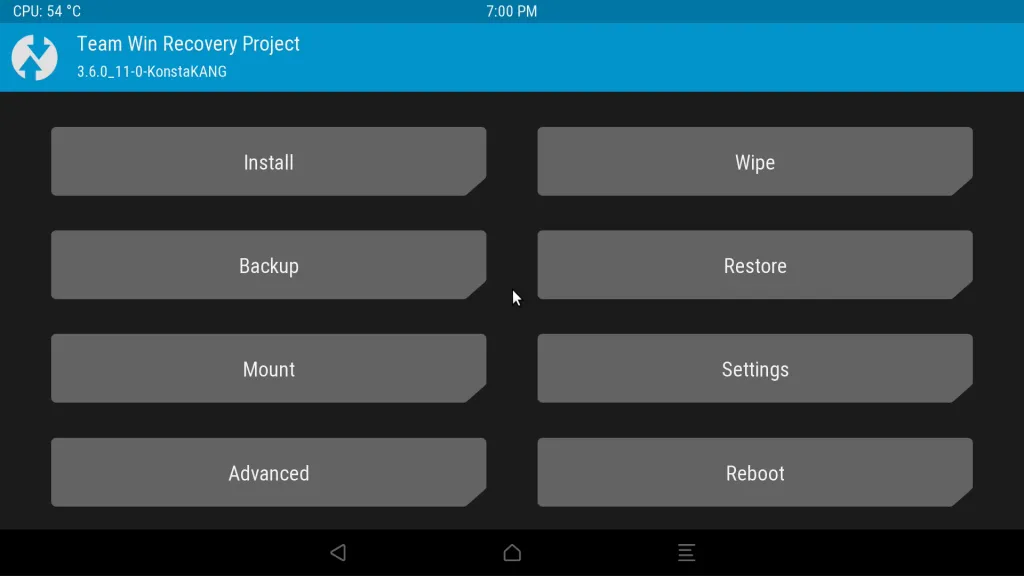
\includegraphics[width=0.9\linewidth,height=68mm,keepaspectratio]{img/p02-05-recovery-mode.png} %CHKTEX 8
		\caption{LineageOS en modo de recuperación}
		\label{fig:recovery-mode} %CHKTEX 24
	\end{subfigure}%
	\begin{subfigure}[b]{0.5\linewidth}
		\centering
		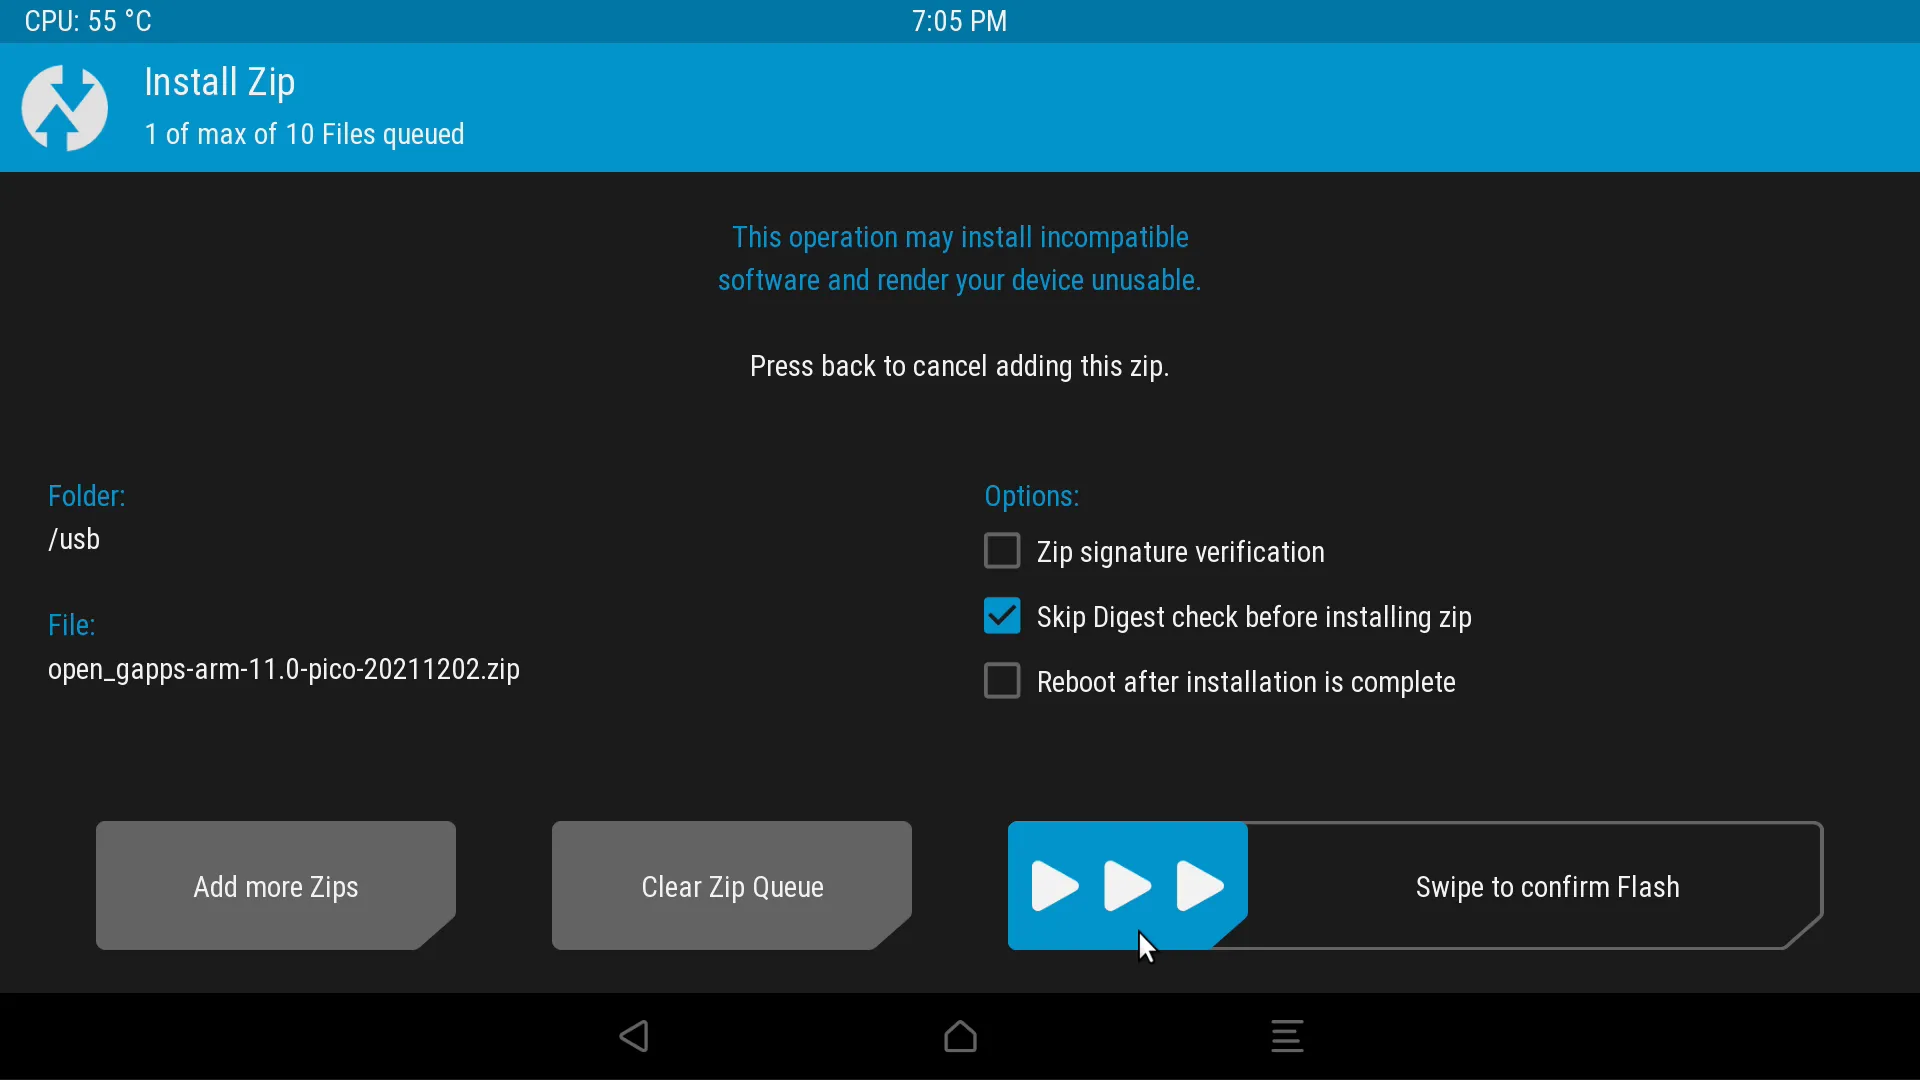
\includegraphics[width=0.9\linewidth,height=68mm,keepaspectratio]{img/p02-05-nikgapps-install.png} %CHKTEX 8
		\caption{Confirmación de instalación de NikGapps}
		\label{fig:nikgapps-install-confirm} %CHKTEX 24
	\end{subfigure}
	\caption{Instalación de NikGapps}
	\label{fig:nikgapps-install} %CHKTEX 24
\end{figure}

\begin{figure}[H]
	\centering%
	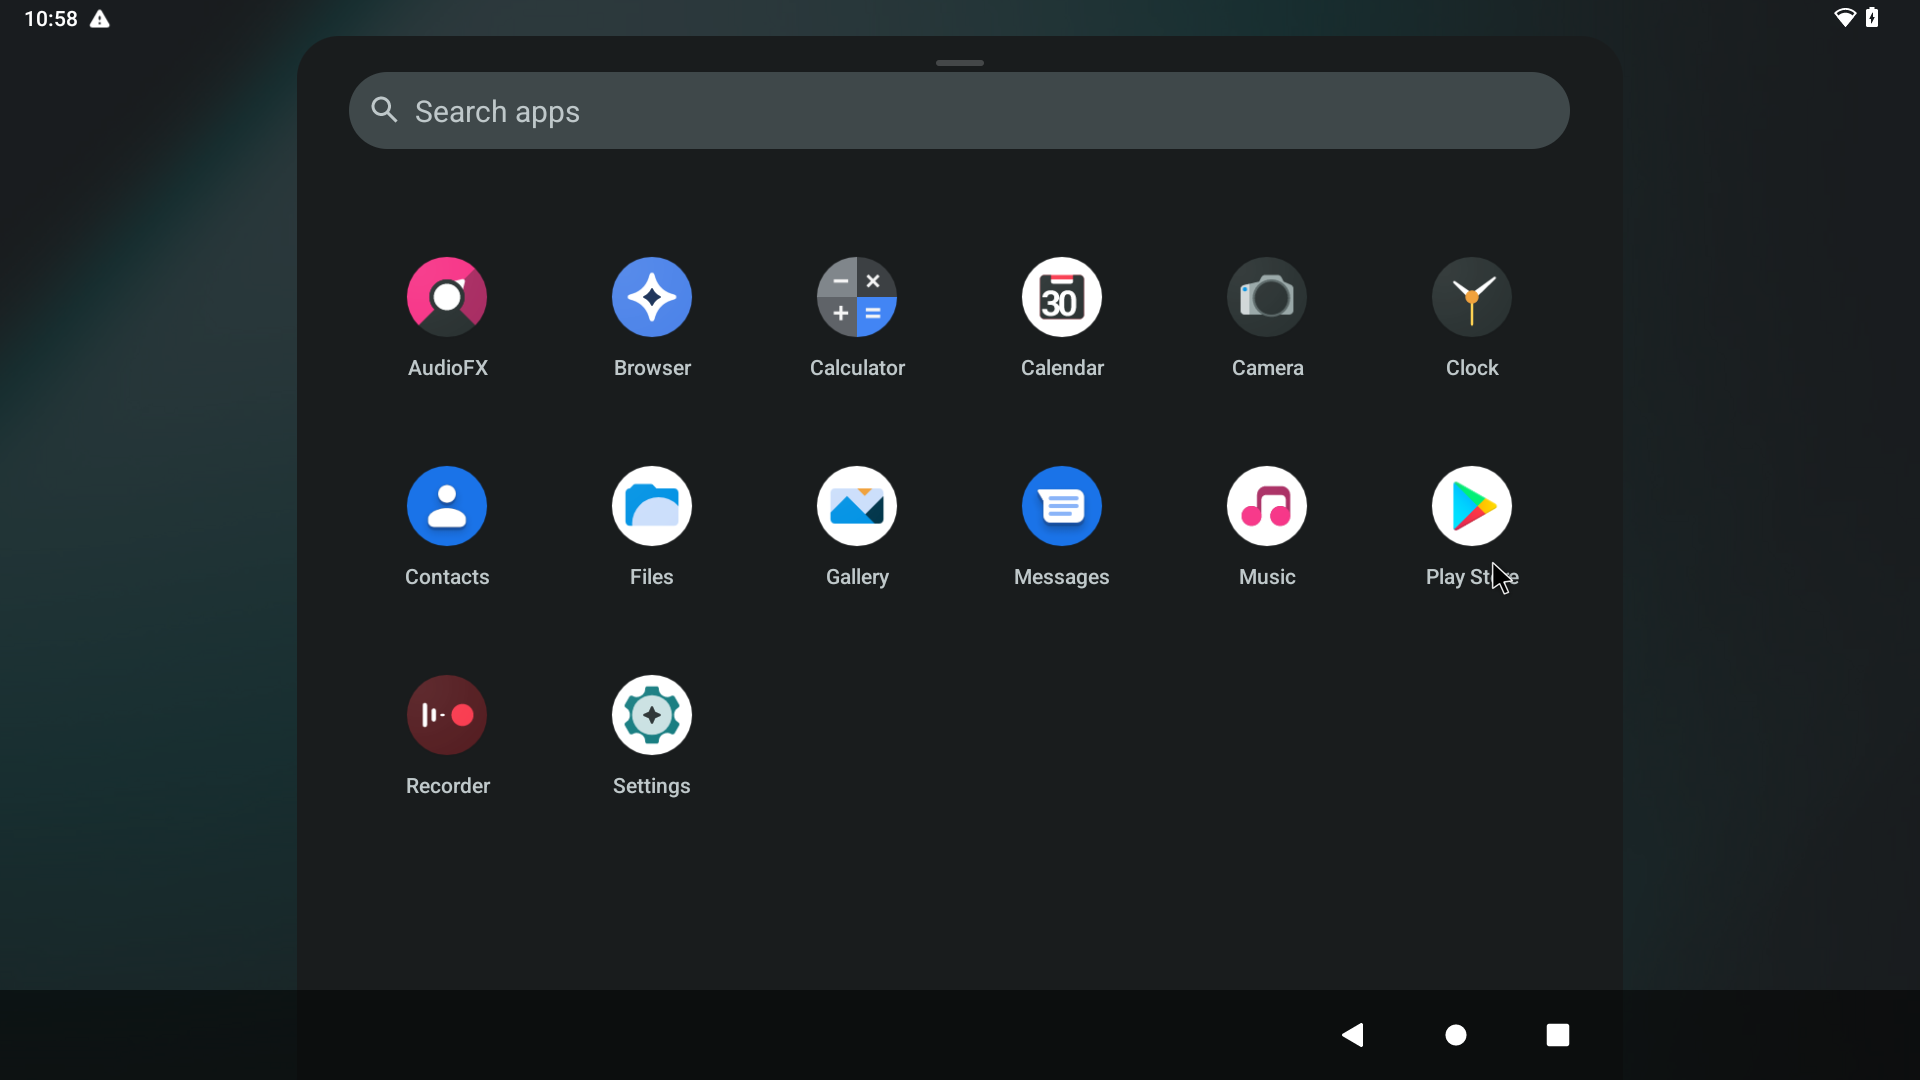
\includegraphics[width=0.9\linewidth,height=68mm,keepaspectratio]{img/p02-06-playstore.png} %CHKTEX 8
	\caption{\emph{Google Play Store} instalada}
	\label{fig:playstore} %CHKTEX 24
\end{figure}

\end{document}
